 \documentclass[a4paper, 11pt]{report}
\usepackage{graphicx}
\usepackage{listings} 
\usepackage{subcaption}
\usepackage[titletoc,title]{appendix}
\begin{document}


\chapter*{Preface}
\addcontentsline{toc}{chapter}{Preface}

This thesis is written in order to complete our master education in electronics and ICT engineering at UHasselt Belgium. The development and writing of this thesis has been done in the Tampere University of Technology, Finland. K. Aerts was the supervisor of our home university, Prof. J. Nurmi and PhD student K. Wang supervised us during the exchange period. \\\\
After several meetings with our supervisors we had a solid idea of what the thesis should be about and what the research question should be. We had some major problems with multiple software versions,  but thanks to dedicated research and trial and error we were able to fix all of these issues.\\
We would like to thank our supervisors to contribute in our work and keep us motivated along the whole experience.\\\\
Thanks, to all our family members who visited us here in Finland to provide us with some comfort after surviving the cold winter and to all new friends we met here. Without the other exchange students, this experience would not have been this great.\\\\\\
Lander Beckers\\
Henning Lakiere\\\\\\
Tampere, 02/06/2017


\chapter{Theoretical background}

\section{parallel computing}
	\subsection{What is parallel computing}
The problem when facing large calculations is that they require a lot of computing power and thus time. Performing these calculations can be done with two types of computation, serial and parallel computing. Serial computing means, you have one compute unit (e.g. a single core CPU) available that performs all instructions on a certain set of data. This set of data will be broken into multiple smaller subparts that will be solved by a certain instruction. The single compute unit performs the instruction on every subpart in order to solve the whole part as shown in figure \ref{fig:SerialC} \cite{barney2012parallel}.
	\begin{figure}[ht]
		\centering
		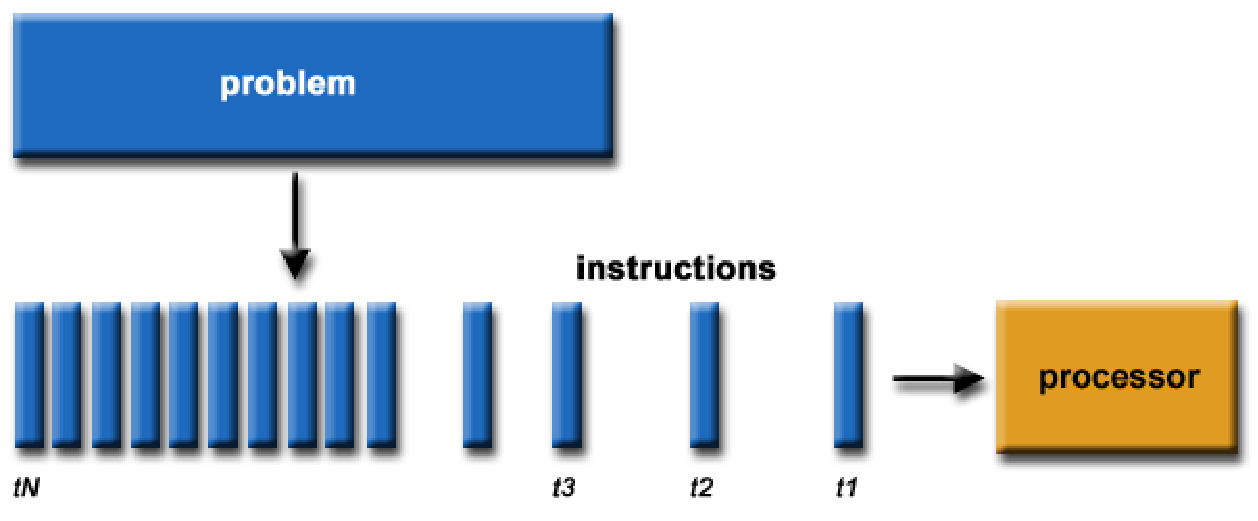
\includegraphics[scale=.4]{images/serialProblem.pdf}
		\caption{Workflow serial computing}
		\label{fig:SerialC}
	\end{figure}

Parallel computing, on the other hand, is the simultaneous use of multiple compute units, or a compute resource, to solve a computational problem. This compute resource can be a CPU with multiple cores, a combination of a CPU with different compute accelorators such as a GPU or even a whole network of computers and servers. We break apart the main problem in smaller subproblems as we did with serial computing. Now, since there are multiple compute units, we can distribute the subproblems among all these compute units. Every unit can now perform an instruction on their given subproblem simultaneously as shown in figure \ref{fig:ParallelC}.
	\begin{figure}[ht]
		\centering
		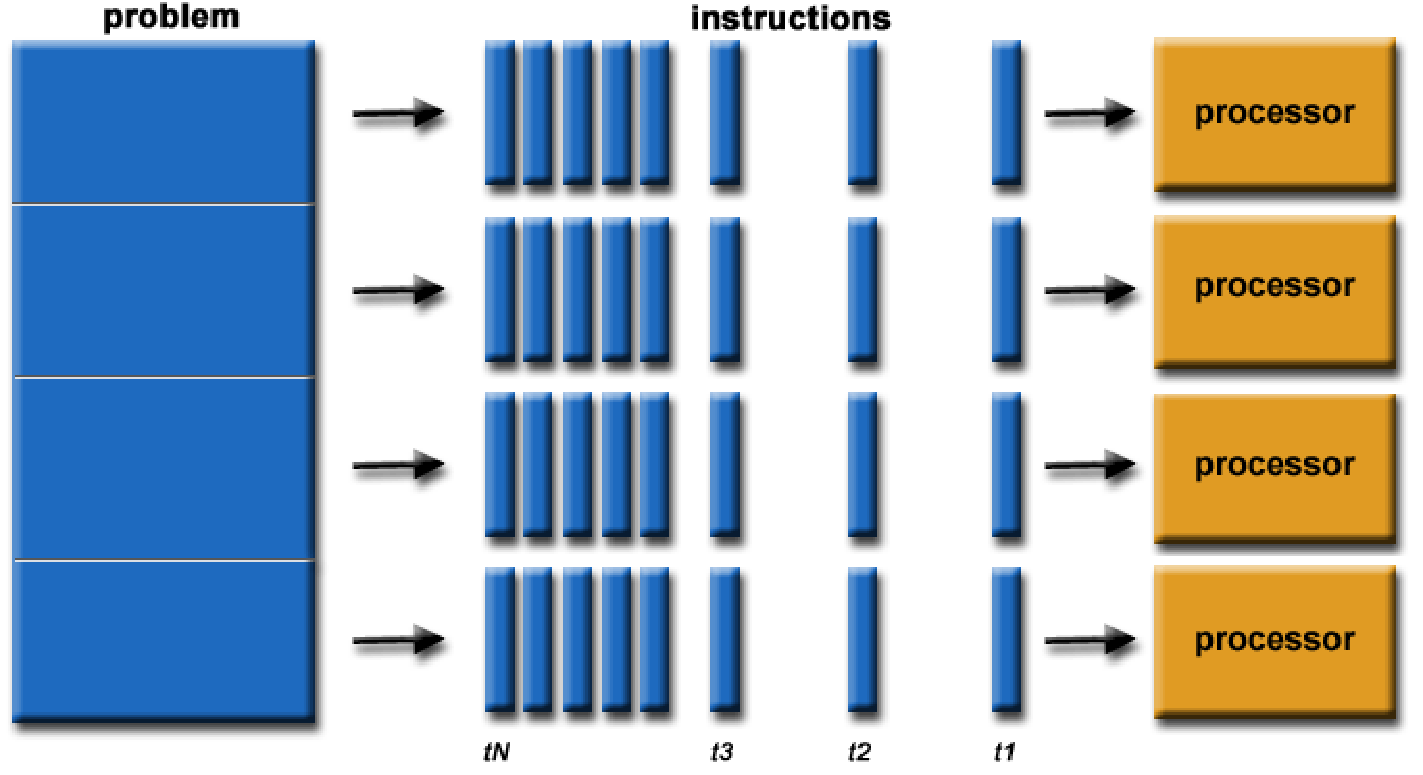
\includegraphics[scale=.4]{images/parallelProblem.pdf}
		\caption{Workflow parallel computing}
		\label{fig:ParallelC}
	\end{figure}
With multiple compute units executing one task, we will shorten the completion time and even have a potential cost saving. It also allows us to solve larger/complex problems since a single computer could suffer from limited memory. And last, we are able to access non-local resources in a network that would not be accessible from a local computer.

It is easy to conclude that the concept of parallel computing was to have a more efficient way to handle large sets of data such as huge databases, images or simulations that involve large datasets. It is also easier to deal with complex data for example algorithms \cite{barney2012parallel}.

	\subsection{Classification of parallel computing}
Parallel computing systems can be separated into different classes. According to Flynn's taxonomy, we can roughly place any of these systems in one of the four classes. This classification was first studied by Michael Flynn in 1972 \cite{Unit2COPC}. The classifications are determined by two factors: instruction stream and data stream which both have two possible states being single or multiple. Figure \ref{fig:flynnTaxonomy} represents a the four possible classes from the Flynn's taxonomy \cite{barney2012parallel}.

	\begin{figure}[ht]
		\centering
		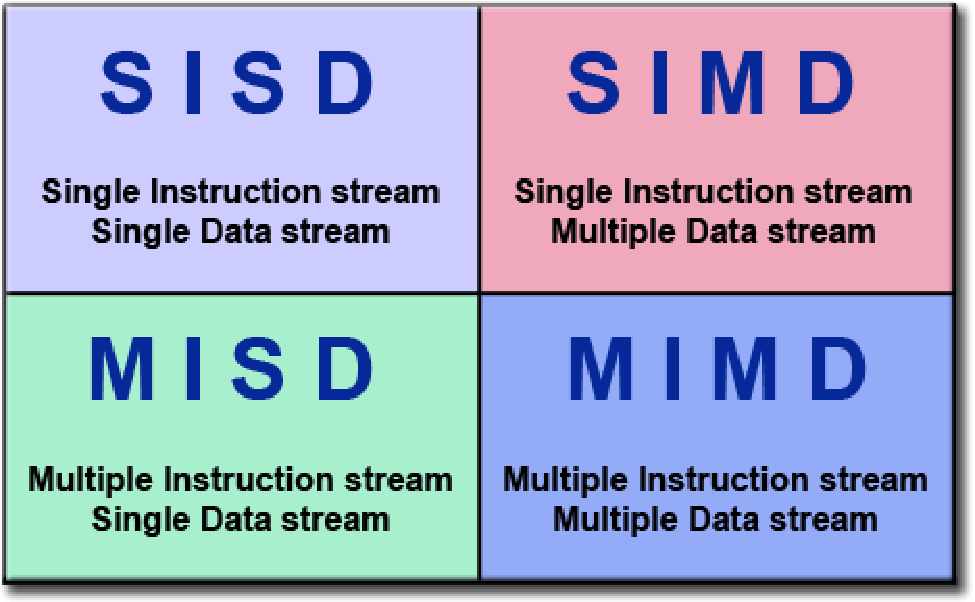
\includegraphics[scale=.5]{images/flynnsTaxonomy.pdf}
		\caption{Four possible classifications according to Flynn's Taxonomy}
		\label{fig:flynnTaxonomy}
	\end{figure}
	
	\begin{itemize}
		\item SISD\\
		
The SISD class will have a single core processor executing a single data stream to operate on data stored in a single memory (figure \ref{fig:sisd}). This means that a parallel compute system cannot be classified as an SISD system, but Flynn's taxonomy was not made for just classifying parallel compute systems. Any traditional single-core processor falls into this category but it is usually old computers or older compute units that can be classified as SISD.
		\item {SIMD}\\
		
Data is distributed amongst multiple processors who all execute the same instruction on this data (figure \ref{fig:simd}). Since we have access to multiple compute units, parallel computing can be categorized in this class. Furthermore, this is the class where we can categorize our subject of the thesis in since we have a large set of data divided over multiple data streams (MD) and only one instruction stream (SI) since all processing units will perform the same instruction on the data. The SIMD class contains the most modern computers, particularly those with a graphics processor unit (GPU).
		\item MISD\\
		
Each processing unit operates on the data independently via separate instruction streams while a single data stream is fed into multiple processing untis (figure \ref{fig:misd}). This class knows very few applications. An example of an application is the use of multiple cryptography algorithms attempting to crack a single coded message.
		\item MIMD\\
		
This time every processing unit is able to execute a different instruction stream on a different data stream (figure \ref{fig:mimd}). This means that any instruction can be applied on any data package for every compute unit. Most supercomputers, networked parallel computer clusters and "grids" can be classified as a MIMD compute system. Also, many MIMD architectures include SIMD execution sub-components.
		\end{itemize}
\begin{figure}[ht]
	\centering
	\begin{subfigure}[t]{0.4\textwidth}
		\centering
		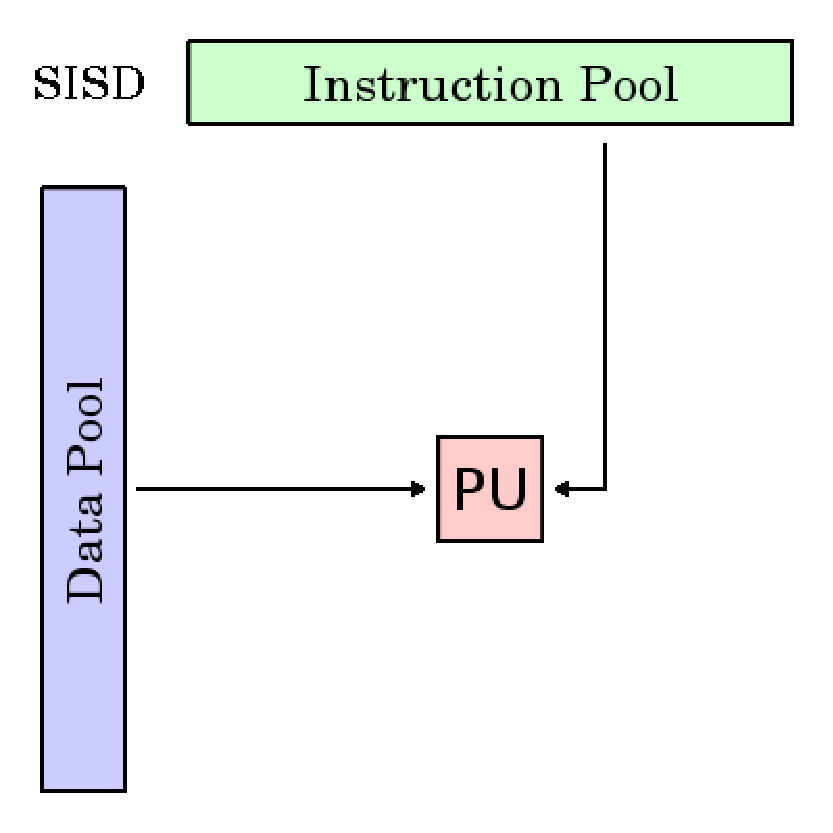
\includegraphics[scale=.3]{images/sisd.pdf}
		\caption{SISD}\label{fig:sisd}
	\end{subfigure}
	\begin{subfigure}[t]{0.4\textwidth}
		\centering
		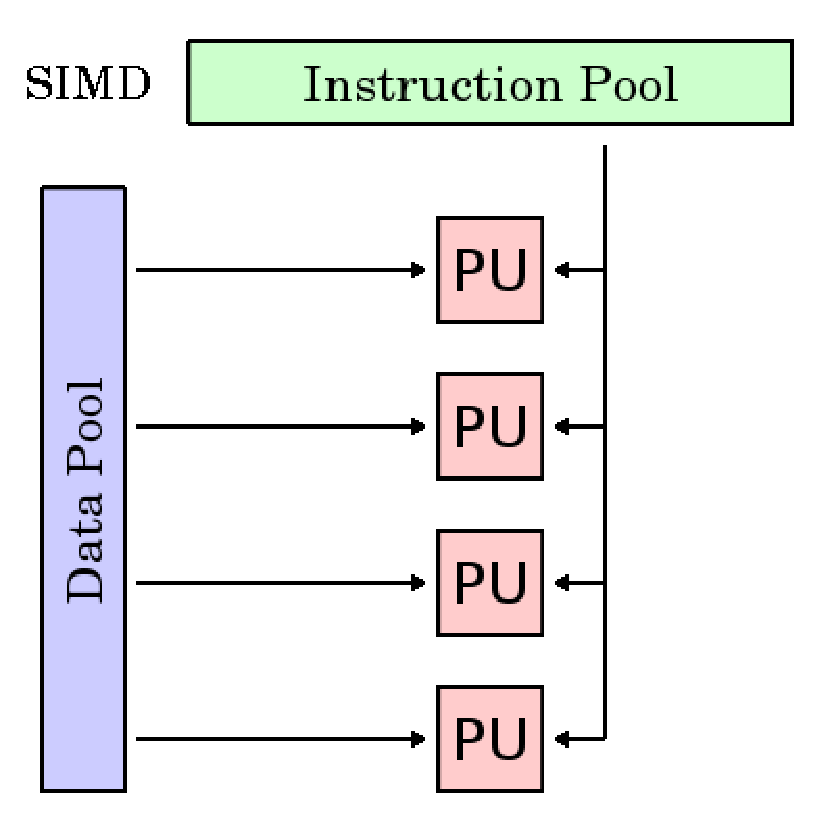
\includegraphics[scale=.3]{images/simd.pdf}
		\caption{SIMD}\label{fig:simd}
	\end{subfigure}
	\begin{subfigure}[t]{0.4\textwidth}
		\centering
		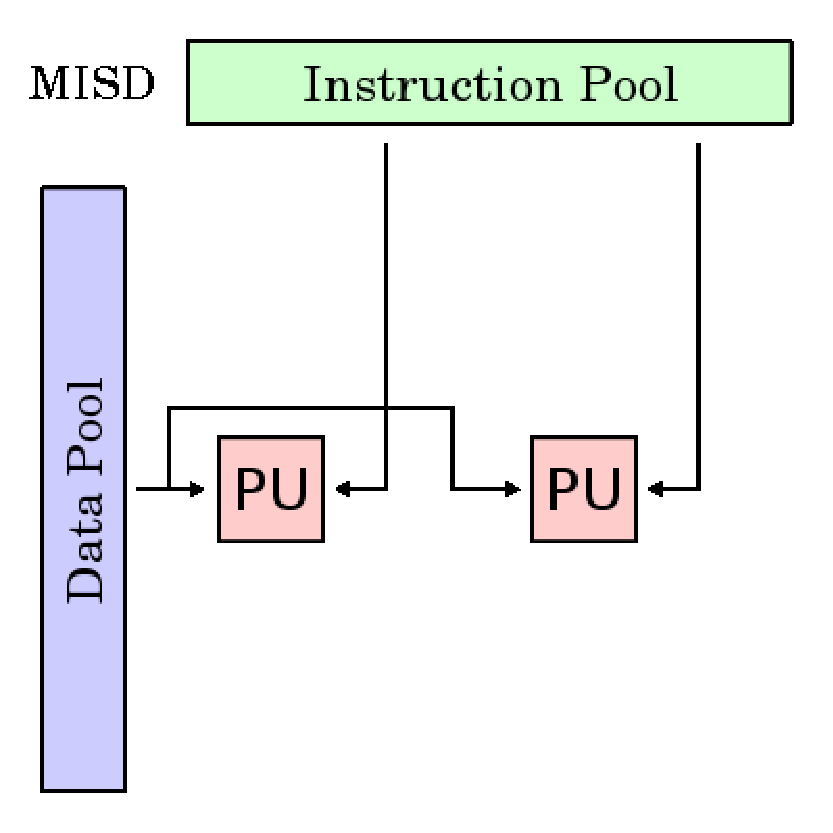
\includegraphics[scale=.3]{images/misd.pdf}
		\caption{MISD}\label{fig:misd}
	\end{subfigure}
	\begin{subfigure}[t]{0.4\textwidth}
		\centering
		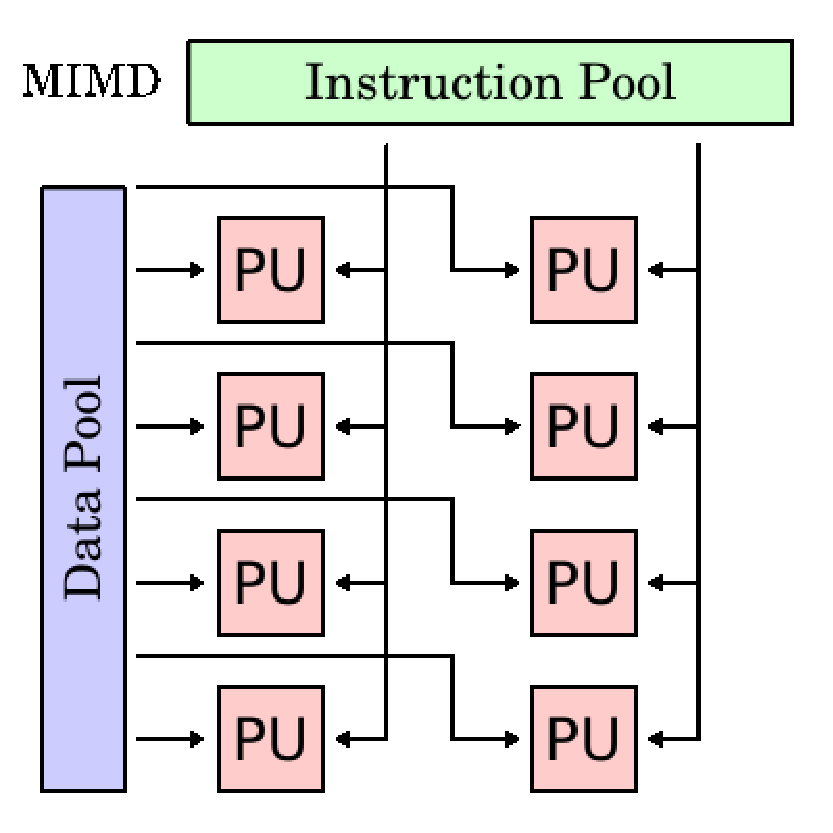
\includegraphics[scale=.3]{images/mimd.pdf}
		\caption{MIMD}\label{fig:mimd}
	\end{subfigure}
	\caption{Architecture classes from Flynn's taxonomy}\label{fig:archFlynnTax}
\end{figure}


\subsection{OpenCL}\label{subsec:OpenCL}

Companies worldwide constantly strive to improve computational performance. They start using GPUs, FPGAs and other compute accelerators that behave as a coprocessor to process parallel workload. In order for these heterogeneous architectures to function properly, we need software that supports heterogeneous computing on hardware platforms from different vendors. To make this possible, developers use toolkits such as Threading Building Blocks (TBB), OpenMP, Compute Unified Device Architecture (CUDA), and others \cite{stone2010opencl}. However, some of the existing toolkits were limited to either only being able to use a single microprocessor family or they did not support heterogeneous computing. OpenCL on the other hand provides a set of easy-to-use abstractions and a wide variety of APIs. OpenCL was developed by the Khronos group as a parallel computing API for Apple's OS X release of Snow Leopard back in 2009. This Khronos group is a mixture of people from different hardware vendors like ATI technologies, Intel, Nvidia to name a few \cite{KhronosMembers}.\\
One of the main reasons companies start using OpenCL is that in the past they would use GPUs, when they should be using FPGAs while others had the problem the other way around. The problem they had is that converting CUDA, which is the parallel computing platform from Nvidia (GPUs), to VHDL is difficult and annoying to do. More reasons on why OpenCL should be used to program FPGAs are listed below \cite{FPGAforDummies}.
\begin{itemize}
	\item {Simplicity and ease of development}\\
	Because most software developers are more familiar with C than low-level HDL language, OpenCL is easy to understand for the vast majority of developers worldwide.
	\item {Code profiling}\\
OpenCL allows you to determine where exactly the performance-sensitive pieces in your code are. This way it is easy to assign these pieces of code to be executed by hardware accelerators as kernels.
	\item {Performance \& Efficiency}\\
Every developer wants to have his software build in the most efficient way to benefit from maximum performance. Due to the FPGA's parallelistic architecture, you only need to generate the logic the device needs to run the software to deliver high performance.
	\item {Code reuse}\\
Since there are multiple devices that are supported by OpenCL, you can reuse your already written code on almost any of the other devices without having to change a thing.
\end{itemize}

\section{Smartphone}
Nowadays, almost everyone has a smartphone. These portable computers allow us to communicate with anyone across the world from almost any place. They can be used as entertainment devices to play music or video games and over the last couple of years even services like trading markets or banking systems have been integrating with smartphones. Furthermore, you can make pictures with them, view all sorts of media, and the list goes on. Since the increasing popularity there has been many companies developing smartphones. But the most common brands are Samsung and Apple accounting for over 37\% of the market shares in 2017 of all smartphone brands \cite{SmartphoneShares}.
	\subsection{Android OS}
Like most communication devices, smartphones need an operating system (OS). While Apple's IPhones use their own OS called iOS, Samsung and many other smartphone manufacturers use the Android OS that was developed by Google. With a whopping 81,7\% worth of market shares at the end of 2016, Android is definitely one of the market leaders when it comes to smartphone operating systems \cite{OSShares}.\\
One of the main features of smartphones are applications or apps short. Google's Play Store has over a million apps available for almost any Android device. Unlike Apple's App Store, basically anyone can upload their own apps on Google's Play Store. To upload apps as a developer for everyone to download and use you pay a one-time fee of 25\$ to Google. Making apps on the other hand is free. Most apps are written in Java and there are multiple integrated development environments (IDE) available for the Android platform. The official IDE for Android is Android Studio which is described in the next section. Other IDEs available are AIDE (HTML, C, C++), Xamarin (C\#) and many others.
	\subsection{Android Studio}
Android Studio is the official IDE where you can develop apps for phones with an Android OS. Its main programming language is Java but since Android Studio 2.2 it is possible to write and use C and C++ code by compiling it into a native library. With the Java Native Interface (JNI) you can call the C/C++ functions in your native library. Furthermore, Android Studio splits up front and back end of the application giving the developer a nice clean overview of the whole project. The front end can be edited through coding or with a visual interface where you can pick and place your required objects in a layout. The front end design is an xml-file that is attached to an activity. This activity is part of the back end where you write your code in order to interact with the front end of the application.

\section{Bluetooth}
Bluetooth is a form of wireless communication that was developed in 1994 by Ericsson Mobile in Sweden. It is a radio frequency (RF) technology using the 2.4GHz industrial, scientific and medical (ISM) band, the same band where you can find ZigBee and WiFi aswell. It can be used to transmit data or voice communication over short distances. Bluetooth radios can be found in nearly every new smartphone and laptop device. It is easy to use, to setup and it has a lot of applications, for example hands-free devices, home heating systems, entertaining devices and so on. Bluetooth is designed to be low cost, for about 5-10\$ per unit. The down side of this is the short connection range and the limited transmission speed of around 780 kb/s \cite{bluetoothTech}.\\

	\subsection{Bluetooth benefits}
The introduction of Bluetooth allowed for many new applications in several areas. Even today it is still widely used, mostly for multimedia devices, keyboards, mices, printers. The following list explains some benefits for three general areas:
		\paragraph{Data and voice acces points.}
Bluetooth allows a wireless connection between devices through which they can communicate. With Bluetooth, the devices are able to transmit voice and data packages in real-time.
		\paragraph{Cable replacement.}
Some wired connections between devices require special cables or adapters. Bluetooth eliminates this hassle since any device can connect to another with the right communication protocol. The range of this connection is approximately 10m and doesn't require the devices to be in line of sight. With an optional amplifier the range can be extended to 100m.
		\paragraph{Ad hoc networking.}
Devices with a Bluetooth radio can establish instant connections with each other as soon they come into range.


	\subsection{Master, slave and piconet}
For a Bluetooth connection to exist, there has to be at least one master and one slave device. They use what is called the master/slave model. A master device can be connected to up to seven slave devices while a slave can only connect to one master device. A network of one master and one to seven slaves is called a piconet. The master device will coordinate all the communication throughout the piconet. All slave devices are allowed to exchange data with the master device when granted premission, but cannot communicate with other slaves in the piconet. The connection between each device is encoded and protected to prevent other devices from eavesdropping and to prevent interference between other devices. Furthermore, in order for these devices to connect with each other, they require the same communication protocol. A device in one piconet can also exist as part of another piconet and can function as either a slave or a master in each piconet. This form of overlapping is called a scatternet \cite{introBluetooth}. An example of two piconets forming a scatternet is shown in figure \ref{fig:scatternet}.

	\begin{figure}[ht]
		\centering	
		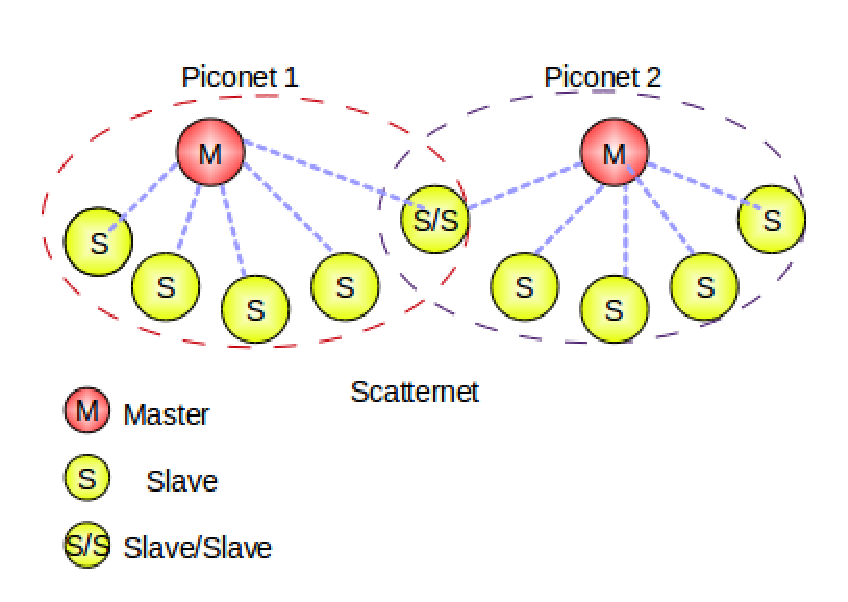
\includegraphics[scale=0.60]{images/scatternet.pdf} 
		\caption{Piconets and Scatternets}\label{fig:scatternet}
	\end{figure}

The piconet/scatternet allows the devices to share the same physical area, allowing the network to make efficient use of the bandwidth. A Bluetooth system can use up to 79 different frequencies using a frequency hopping (from 2.402 to 2.480 GHz) \cite{bluetoothStack} scheme with a carrier spacing of 1MHz. This allows a bandwidth of 80MHz. Without frequency hopping scheme, every single channel would have a bandwidth of 1MHz at their disposal. With frequency hopping, the sequence will define a logical channel. This allows to have an available bandwidth of 1MHz at any given time, with a maximum of eight devices sharing the bandwidth. This 80 MHz bandwidth can be shared by several different logical channels. Though, this can cause signal collisions when devices in different piconets, on different logical channels have the same hop frequency at a given time. Signal collisions degrade the performance, so we can state that the more piconets we have, the more collisions occur, the lower our total performance will be \cite{introBluetooth}.

	\subsection{Protocol architecture}
The Bluetooth protocol architecture consists of four basic layers: core protocols, cable replacement, telephony control protocols and adopted protocols. Figure \ref{fig:bluetoothStack} shows the architecture of the Bluetooth protocol stack.
	\begin{figure}[ht]
		\centering
		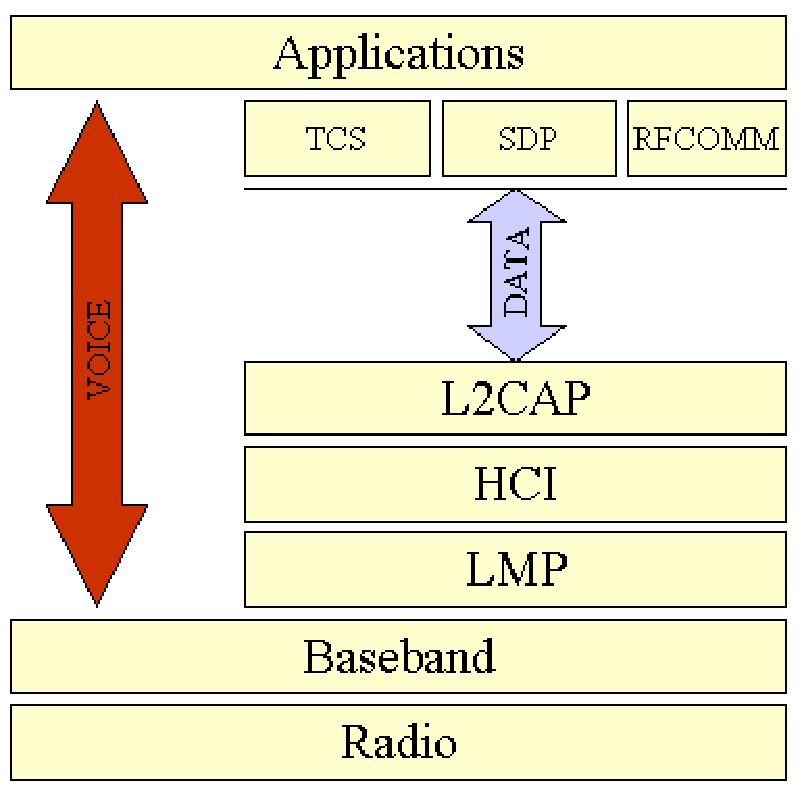
\includegraphics[scale=0.5]{images/bluetoothStack.pdf}
		\caption{Bluetooth protocol stack}\label{fig:bluetoothStack}
	\end{figure}

		\paragraph{Core protocols.}
The core protocol is a five-layer stack. Every layer in the stack has its own responsibilities that are mentioned below.

		\begin{itemize}
			\item The \textit{radio} layer is the wireless connection that specifies certain details about the air interface, including frequency, the use of frequency hopping, modulation scheme and transmit power. 
			\item The \textit{baseband} layer is responsible for the packet transmission to the radio layer. As mentioned before this data can contain data or voice packages. For the data packages, asynchronous connectionless (ACL) links are used while voice packages are transmitted with synchronous connection-oriented (SCO) links. The baseband layer maintains both ACL and SCO links. It is important for data packages to be transmitted correctly to maintain data integrity, while it is not a problem in case some voice packages get lost. That is why SCO packages are never retransmitted. If you would retransmit voice packages, every next package would suffer from a time delay restraining us from having real-time communication.
			\item The \textit{Link manager protocol (LMP)} uses the links setup by the baseband and manages the connection between Bluetooth devices. Furthermore, it is responsible for monitoring service quality, security aspects such as device authentication, encryption plus the control and negotiation of baseband packet sizes.
			\item The \textit{Host controller interface (HCI)} is the layer between the hardware and the software. The L2CAP layer and the layers above it are implemented in the software while all other layers under the HCI (LMP, baseband, radio) are part of the hardware. The HCI driver acts as a physical bus that connects the hardware with software. It is possible to access the L2CAP layer directly by the application making it easier for application programmers. This makes the HCI, in some cases, an unnecessary component.
			\item The \textit{Logical link control and adaptation protocol (L2CAP)} receives application data and transforms this to the Bluetooth format. Furthermore, Quality of Service (QoS) parameters are exchanged at this layer \cite{bluetoothStack}.
			\item According to \cite{bluetoothStack}, the \textit{Service discovery protocol (SDP)} is not a part of the Core protocols. Though, it contains all the information, services and charasteristics  in order to establish a connection between two or more Bluetooth devices. The LMP uses the SDP's first to find out what services are available from the acces point. Then information from the SDP is obtained by the LMP to create a L2CAP channel.
		\end{itemize}
		
		\paragraph{Cable replacement.}
The RFCOMM seen in figure \ref{fig:bluetoothStack} is the cable replacement protocol. It is a virtual serial port that is designed to replace cable technology. Serial ports are common types of communication interfaces used with computing and communication devices \cite{introBluetooth}. So with RFCOMM we eliminate the need for serial ports for communication between two devices, assuming both are equiped with a Bluetooth radio. 
EIA-232, once known as RS-232, is a widely used serial port interface standard. The RFCOMM will provide binary data transport and has to emulate EIA-232 control signal to the baseband layer.

		\paragraph{Telephony control protocols.}
Telephony control specifications (binary) or TCS BIN, is a bit-oriented protocol that is necessary to define the call control services in order to establish speech or data calls between the Bluetooth devices.

		\paragraph{Adopted protocols.}
Adopted protocols are protocols developed by other organizations. They are "adopted" into the overall Bluetooth architecture. They are usually standard protocols well known in applications other than Bluetooth. Bluetooth's strategy is to only invent necessary protocols and use existing standard protocols whenever possible. The following standards are the adopted protocols:

	\begin{itemize}
		\item The \textit{PPP}, or point-to-point protocol is as a internet standard protocol for transporting IP datagrams over point-to-point links.
		\item \textit{TCP/UDP/IP}, are the foundation protocols of the TCP/IP protocol suite.
		\item \textit{The object exchange protocol}, or OBEX, is a session level protocol made by the Infrared Data Association (IrDA). It is used for exchaning objects. OBEX comes with quite similar funcionalities as HTTP, but in a simpler way. There is also a model included in OBEX that is used for the representation of objects and operations.
		\item Bluetooth also adopts the wireless application environment \textit{WAE} and the wireless application protocol \textit{WAP} into its architecture.	
	\end{itemize}


\section{Web sockets}
Web sockets are used for fast, real-time communication between a server and a client. The HTTP model, which is also a communication protocol between a server and a client, allowed the client only to request data from the server, while the server was only able to fulfill these requests. Web sockets on the other hand, allow bidirectional communication  between the server and the client. This means both client and server can request data and also respond to these requests. The main point of web sockets is to have true concurrency and to focus on the optimization of performance when it comes to communication and exchanging data. The web socket protocol that will be discussed is also known as the RFC6455 model \cite{RFC6455}.

	\subsection{WebSocket communication}\label{subsec:WebSocketCom}
		\paragraph{Handshake.}
To communicate over web socket, the server and the client first have to connect with each other. The establishment of a web socket connection is done by a web socket handshake. Handshaking is the exchange of information between two devices and the agreement about which protocol will be used to exchange data after the connection is established. A well known example of this is the TCP three-way-handshake. The client sends a synchronization message (SYN) to the server as a request to synchronize with the server. If the server receives this message and allows the client to synchronize with it, it will send a similar SYN message and an acknowledgement message (ACK) to let the client know that it has received the request. When the client receives the SYN-ACK message, it will send an ACK message back to the server to acknowledge that it has received the server's message. The TCP connection is established whenever the server receives the ACK message from the client.\\
The web socket handshake is quite similar. The client sends a handshake request to the server, and the server will respond with a similar handshake request as seen in figure \ref{fig:WebSocketHandshaking}. The desktop, smartphone and tablet in figure \ref{fig:WebSocketHandshaking} represent the clients that are connected to the server. The handshake request from the client-side is shown in listing \ref{lst:clientHandshake}, while the response from the server is shown in listing \ref{lst:serverHandshake}.
	\begin{figure}[ht]
		\centering
		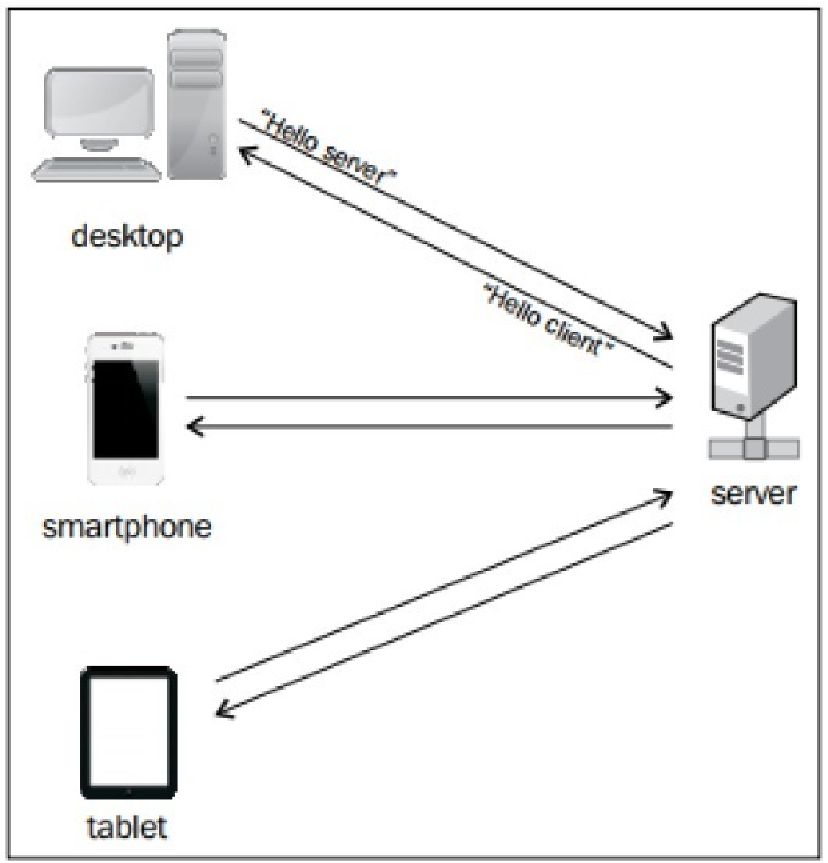
\includegraphics[scale=0.5]{images/server.pdf}
		\caption{Web socket handshaking}\label{fig:WebSocketHandshaking}
	\end{figure}
	\begin{lstlisting}[caption={Client's request for WebSocket handshake},captionpos=b, label={lst:clientHandshake}, language=c, float=h]
  1| GET /chat HTTP/1.1
  2| Host: example.com:8000
  3| Upgrade: websocket
  4| Connection: Upgrade
  5| Sec-WebSocket-Key: dGhlIHNhbXBsZSBub25jZQ==
  6| Sec-WebSocket-Version: 13
	\end{lstlisting}\\
Listing \ref{lst:clientHandshake}, the handshake request from the client, is a pretty standard HTTP request. It is built with multiple headers, some of which are mandatory for the request to be valid. If one of the headers is not understood, the server will reply with "400 Bad Request" and it will close the socket afterwards. In some cases, it will also give a reason why the handshake failed, although browsers do not display these messages. If there is a problem with version numbers, the server adds a "Sec-WebSocket-Version" header in the HTTP response that contains the version it understands \cite{BadRequest}.
	\begin{lstlisting}[caption={Server's response for WebSocket handshake},captionpos=b, label={lst:serverHandshake}, language=c, float=h]
  1| HTTP/1.1 101 Switching Protocols
  2| Upgrade: websocket
  3| Connection: Upgrade
  4| Sec-WebSocket-Accept: s3pPLMBiTxaQ9kYGzzhZRbK+xOo=
  5|
	\end{lstlisting}
When the server receives a request handshake from a client with all the necessary headers, it will reply with a HTTP response as shown in listing \ref{lst:serverHandshake}. The "Sec-WebSocket-Accept" header is derived from the "Sec-WebSocket-Key" header from the client's handshake request. To get it, we combine the "Sec-WebSocket-Key" header and "258EAFA5-E914-47DA-95CA-C5AB0DC85B11" together. The second string is "a magic string". A magic string is predefined by the developer. It is made in a way where you would not expect it to be received from an input. When the "Sec-WebSocket-Key" header and the magic string are combined, the SHA-1 hash is taken from the result, and the base64 encoding of the hash is returned \cite{BadRequest}. The SHA-1 is a cryptographic hash function, while base64 is a binary-to-text encoding scheme.

		\paragraph{WebSocket URI's}
WebSocket defines two URI schemes. You can either use ws or the wss scheme. The ws (web socket) is a regular connection similar to http. While wss (web socket secure) is a secured connection similar to https. The schemes are built as follows:\\

\indent	ws-URI  = "ws:" "//" host [ ":" port ] path [ "?" query ]\\
\indent	wss-URI = "wss:" "//" host [ ":" port ] path [ "?" query ]\\

The most important components of the ws or wss are the host and its port. The host is determined by the server's IP address, while the port defines which port the server uses for the communication. If there is no specified port, the standard port used for ws is 80, and the standard port used for wss is 443.
		
		\paragraph{Data Frames.}
The main advantage of WebSockets is bidirectional communication. So at any point in time, either the client or the server can send a message. Every data frame that is sent from the client to the server, or vice versa, follows the same format as seen in figure \ref{fig:dataFrame}.

	\begin{figure}[ht]
		\centering
		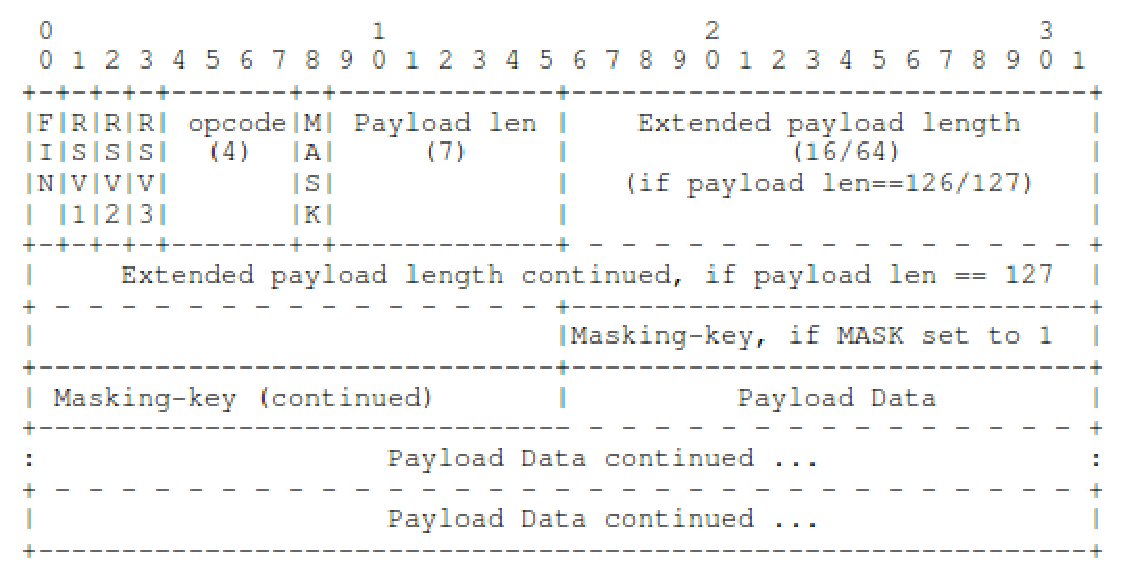
\includegraphics[scale=0.5]{images/WebSocketDataFrame.pdf}
		\caption{Standard WebSocket dataframe format}\label{fig:dataFrame}
	\end{figure}

	\begin{itemize}
		\item {FIN: 1 bit}
	\end{itemize}
Depending on the value of this bit, it either tells the receiving end whether or not this is the final fragment of the message. If the bit equals "0", it is not the last fragment and the receiver will continue listening for more fragments. If the bit equals "1", it means it is the last fragment of the message and the server will consider the message being delivered.
	\begin{itemize}
		\item {RSV1, RSV2, RSV3:  1 bit each}
	\end{itemize}
All of these bits are reserved for WebSocket extensions. They should be "0" unless the client and server negotiated on whether or not a specific extension requires the use of any of the three bits. If any of these three bits is not zero while the client did not negotiate on any of these bits being non-zero, the receiving end will "fail" the WebSocket connection.
	\begin{itemize}
		\item {Opcode:  4 bits}
	\end{itemize}
These 4 bits will define how the receiving end should interprete the data. If the receiving end does not understand the opcode it will, as in the previous case, "fail" the WebSocket connection. The information about the different opcodes is found at \cite{opcode}.
	\begin{itemize}
		\item[] {x0: continuation frame; this frame contains data that should be appended to the previous frame}
		\item[] {x2: binary frame; this frame (and any following) contains binary data}
		\item[] {x3 - x7: non-control reserved frames; these are reserved for possible WebSocket extensions}
		\item[] {x8: close frame; this frame should end the connection}
		\item[] {x9: ping frame}
		\item[] {xA: pong frame}
		\item[] {xB - xF: control reserved frames}
	\end{itemize}
	\begin{itemize}
		\item {Mask bit: 1 bit}
	\end{itemize}
This bit tells wether or not the frame uses a mask. If this bit is set to "1", a masking key is included in the message.  This masking key is used to unmask the data in the payload. Every frame that is sent from the client to the server must have this bit set to "1".
	\begin{itemize}
		\item {Payload length: 7 bits, 7+16 bits, 7+64bits}
	\end{itemize}
The seven bits determine the length of the payload. If these seven bits equal 126, or "1111110", the actual length is determined by bits 16 to 31 (so 16 extra bits). These are the following 2 bytes. If the seven bits equal 127, or "1111111", the actual length is determined by bits 16 to 79 (so 64 extra bits). These are the following 8 bytes.

	\begin{itemize}
		\item {Masking key: 4 bytes}
	\end{itemize}
As mentioned previously, this field only exists if the mask bit is set to one. All the messages who have this field set to one, are masked by a 32-bit value. If the mask bit is set to zero, there will be no masking key in the first place.

	\begin{itemize}
		\item{Payload data: x+y bytes}
	\end{itemize}
The payload data is the combination of the extension data and the application data. These two are listed below.

	\begin{itemize}
		\item{Extension data: x bytes}
	\end{itemize}
The extension data is non-existent unless it was negotiated on the opening handshake between the server and the client. As mentioned earlier, the RSV1-3 bits are responsible for these extensions. Any extension that has been negotiated by the client and server must have a specified length of the "Extension data". It can also tell the receiving end on how to calculate this length. As said previously, the extension is part of the total payload data.
	
	\begin{itemize}
		\item{Application data: y bytes}
	\end{itemize}
The application data contains the actual data that has be to transmitted. It takes up the remaining space in the frame after any extension data. The application data is, like the extension data, part of the payload data.

	
	\chapter{Implementation}
	
	
\section{Communication protocol}
If we want to communicate between the devices, we have to define a set of rules that each of the devices have to follow. These rules should be made in a way that 100\% of the transmitted data will arrive at the receiving end. For example, if data gets lost through transmission, the device on the receiving end will not receive all the necessary data. This can be prevented by adding a checksum that is different then from all other receivable data. If the received message looks incorrect, the receiving device has to respond by asking to resend this piece of data. We are trying out two different communication technologies so we have to set up a communication protocol for each one of them since they both have different performance aspects. To clarify future images, matrix A and B are the matrices sent to the Soc in order to calculate their multiplication. Matrix C is the calculated matrix send back to the phone.

	\subsection{Bluetooth communication protocol}\label{subsec:bluetoothProtocol}
To define a set of rules we first analyzed how good the Bluetooth transmission is. We did some testing and came to the conclusion that there was quite a lot of data loss. We first tried sending eight characters at once but nearly 80\% of the time there was atleast one of the characters missing. Missing one number would mean that the matrix we need is incorrect and this would lead to an incorrect outcome. We did some further testing and realized it was the best option to send four numbers at a time. With this we can set up our first rule. The first rule being, we let both devices know that they should always send four numbers at once. Both devices also know they should receive four numbers. If this is not the case we have to resend the message.
In order to make sure all characters would arrive at the receiving end, we added an extra character ':' at the end of each message. This character lets the receiving end know that it is the end of a message. If we would not define the end of a message and a number would be missing, the receiving end would wait for the next number to come through. The problem is that the next number would be part of the next message causing the all numbers to be messed up with each other. An example of a message would look like this: 4372: .\\
Now for the communication, we start off by connecting both devices with Bluetooth. As soon as the devices are connected with each other, the SoC will send message "C" to the Android phone notifying it is ready to receive the two matrices. As soon as the phone receives message "C", it will start sending the first number or in some cases a part of the number. In case the message is received correctly, the SoC sends the message "O" to let the phone know the message was received. Figure \ref{fig:correctMessage} shows an example of how a correct message should look like.

\begin{figure}[ht]
\centering
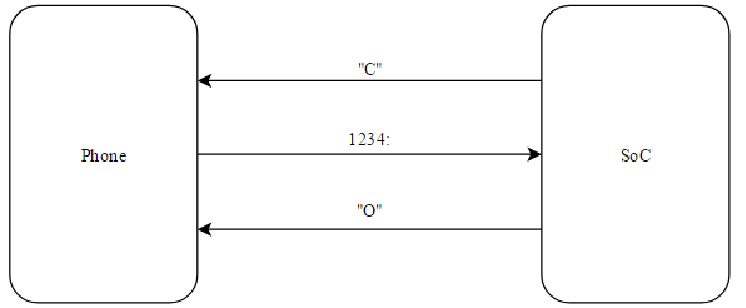
\includegraphics[scale=0.7]{images/CorrectMsg.pdf}
\caption{Correct message transfer}\label{fig:correctMessage}
\end{figure}

In case we are missing a number due to data loss, the receiving end will respond with the message "R" as shown in figure \ref{fig:incorrectMessage}

\begin{figure}[ht]
\centering
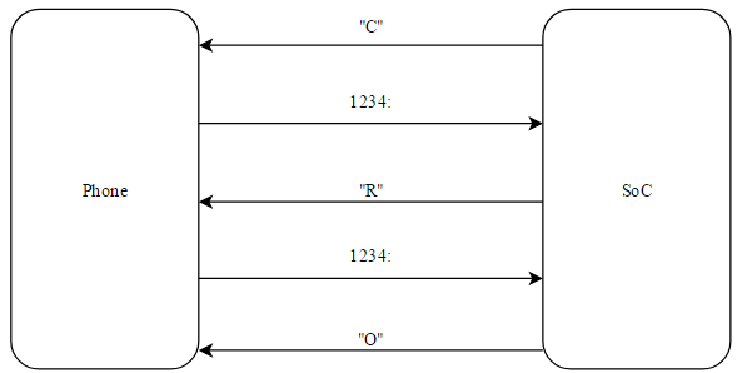
\includegraphics[scale=0.7]{images/IncorrectMsg.pdf}
\caption{Incorrect message transfer}\label{fig:incorrectMessage}
\end{figure}

There is also the possibility of a device not responding to a request. The receiving end is waiting for a response from its request. If the wait time is too long compared to a predefined waiting time, the receiving end will send a message "R" as seen in figure \ref{fig:delayedMessage}.

\begin{figure}[ht]
\centering
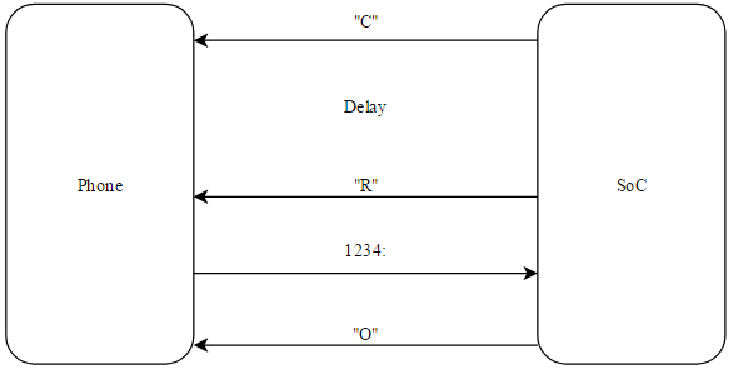
\includegraphics[scale=0.7]{images/DelayedMsg.pdf}
\caption{Delayed message}\label{fig:delayedMessage}
\end{figure}

As for now, we work with square matrices with a predefined size. Both devices know at the start of the session how large both matrix A and matrix B are. This way the SoC can calculate how many numbers it should receive from the phone. Whenever matrix A is transferred succesfully, the Soc will send message "D" to notify the phone it should start sending matrix B (Figure \ref{fig:shiftMatrix}). The same procedures as mentioned above are applied on matrix B as well.

\begin{figure}[ht]
\centering
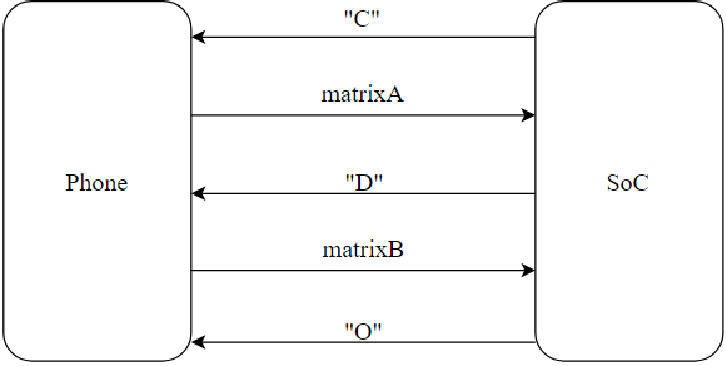
\includegraphics[scale=0.7]{images/ShiftMatrix.pdf}
\caption{Switch matrix message}\label{fig:shiftMatrix}
\end{figure}

When both matrices are transferred, the role of transmitter and receiver are switched. The phone will now act as a receiver while the SoC becomes the transmitter. The SoC will transmit matrix C after doing the multiplication of matrices A and B. For this proces, the previous rules are also applicable. Although this time, the phone will start off by sending a message "C" to notify the SoC that it is ready to receive matrix C. The SoC proceeds by sending the data in the same way as the phone did. Whenever the transmission experiences data loss, the phone will send message "R" to the SoC exactly like the SoC does the other way around.
Message "D" is not used by the phone since there is only one matrix it should receive from the SoC. When the phone received matrix C, the Bluetooth connection between the devices will be suspended.

	\subsection{Web socket communication protocol}\label{subsec:websocketProtocol}
The web socket communication has to achieve the same goal as the Bluetooth communication being transmitting matrix A and B. Depending on the efficiency and performance of this web socket communication we set up a similar set of rules. Compared to Bluetooth, the web socket transmission is much more efficient. We can easily transmit over eight characters without having any data loss. This means that we do not have to send acknowledgement messages like the "O" or "R" message that were necessary with the Bluetooth communication in order to have a solid data transmission.

If we look at subsection \ref{WebSocketCom} under data frames, we see that the payload length of a message can be either 16 or 64 bits. But this does not mean we are limited to sending messages smaller than 64 bits at a time since the socket will just split up the data in seperate messages. This allows us to basically have any message size. Because of limited memory we chose to use integer numbers between 0-99. Next, we decided to combine 4 numbers and make one message with them. The message now contains 4 integers (16 byte). We convert the integers to strings and add a "0"-string in front of numbers that are smaller than 10 to make sure the full message has a constant length of eight characters.

In order to have any communication at all, we start of by connecting both devices through web socket technology. As soon as both devices are connected with each other, the SoC will again start of by sending a message. The message will ask the phone to send matrix A. The phone then will start transferring all data from matrix A to the SoC. Whenever matrix A is transmitted completely, the SoC will ask to transfer matrix B and the phone will send matrix B. After the last number of matrix B being transferred, the SoC will confirm that all data has been received. In figure \ref{fig:Matrices} we can see the exact messages needed from the SoC in order to have a correct communication process. The messages from the phone to the SoC are examples of how the messages could look like. The first message "12345678" would be numbers 12, 34, 56 and 78 being transmitted to the SoC.

\begin{figure}[ht]
\centering
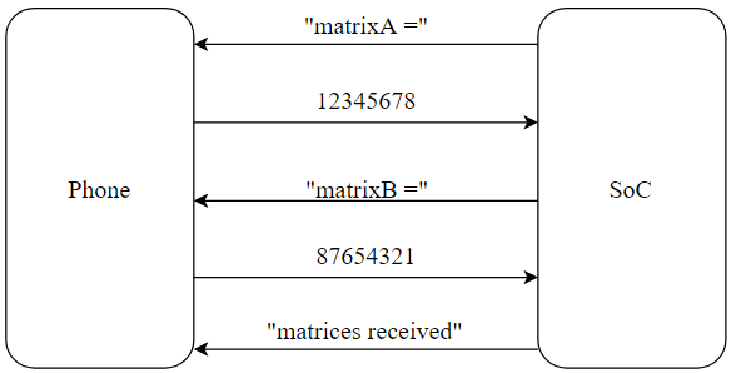
\includegraphics[scale=0.7]{images/webSocketCom.pdf}
\caption{Sending matrix A and B}\label{fig:Matrices}
\end{figure}

After the SoC sends its last message it will start doing the matrix multiplication of matrix A and B with the outcome being matrixC. When the SoC is ready it will send the message "matrixR =" to notify the phone it will start sending over the values within matrix C. Unlike the phone, the SoC will send each number one by one since the number length varies with the size of the matrix. Figure \ref{fig:ResultMatrix} shows both types of messages being send by the SoC. The phone should receive all numbers without having to give any feedback to the SoC. Whenever the full result matrix is transmitted by the SoC, the web socket connection is terminated and the complete process is finished.

\begin{figure}[ht]
\centering
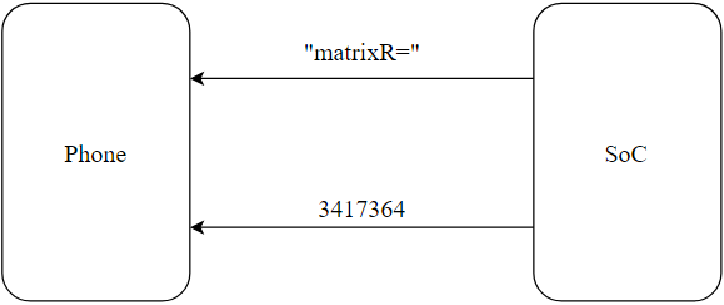
\includegraphics[scale=0.7]{images/webSocketCom2.pdf}
\caption{Sending result matrix}\label{fig:ResultMatrix}
\end{figure}

\section{Android apps}\label{sec:AndroidApps}
The android phone needs proper software in order to function well in our expirement. To build this software we use Android Studio. It is an easy-to-use java environment with a lot of information that can be found on the internet. We will make three different applications using Android Studio. One application to test the matrix mulitplication with the phone itself to compare the speed with the SoC. A second application is responsible for the Bluetooth communication and a third application is used for the web socket communication.

	\subsection{Matrix multiplication}
This app will multiply two square matrices that are filled with random integers converted to strings (see subsection \ref{subsec:websocketProtocol} on why we do this). We start of with creating two matrices. Listing \ref{lst:createMatrix} shows how this is done. We start of by making an array of integers that is "arraySize" large. We start a for loop that will cycle "arraySize" times. In line 4 we create a random integer between value 0 and 99 and put this in the array "matrixA" in the next line. MatrixB is made in exactly the same way.

\begin{lstlisting}[caption={Creating matrix},captionpos=b, label={lst:createMatrix}, language=java, float=ht]
 1| matrixA = new Integer[arraySize];
 2| int random;
 3| for (int i=0; i<arraySize;i++){
 4|   random = (int) (Math.random()*100);
 5|   matrixA[i] = random;
 6| }
\end{lstlisting}
We then go through listing \ref{lst:matrixMultiplicationApp} which is a basic way of multiplying two matrices.
\begin{lstlisting}[caption={Code for matrix multiplication on Android phone},captionpos=b, label={lst:matrixMultiplicationApp}, language=java, float=ht]
 1| t1 = (int) System.currentTimeMillis();
 2| for(int i=0; i<arraySize; i++){
 3|   for(int j=0; j<arraySize; j++){
 4|     sum = 0;
 5|     for(int k=0; k<arraySize; k++){
 6|       sum = sum + matrixA[i*arraySize+k]*matrixB[k*arraySize+j];
 7|     }
 8|     matrixC[i*arraySize+j] = sum;
 9|   }
10| }
11| t2 = (int) System.currentTimeMillis();
\end{lstlisting}

First, we determine the system time and assign this value to t1. In section \ref{sec:matrixMultiplication}, we explain how matrix multiplication works so this should clear up lines 2-10 in the listing above. After the multiplication is finished we determine another system time and assign this value to t2. If we distract t1 from t2, we know how many milliseconds it took to complete the full multiplication. The layout of this app can be seen in figure \ref{fig:app1layout}.

\begin{figure}[ht]
\centering
	\begin{minipage}[t]{0.4\textwidth}
		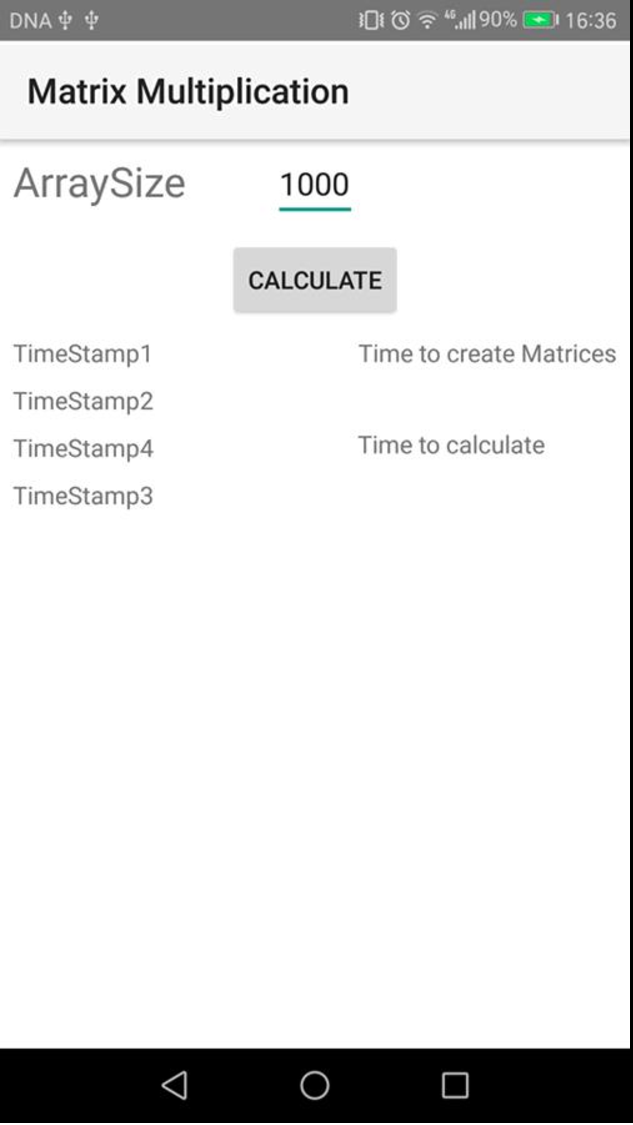
\includegraphics[scale=0.4]{images/app1layout.pdf}
		\caption{Matrix multiplication app}\label{fig:app1layout}
	\end{minipage}
	\begin{minipage}[t]{0.4\textwidth}
		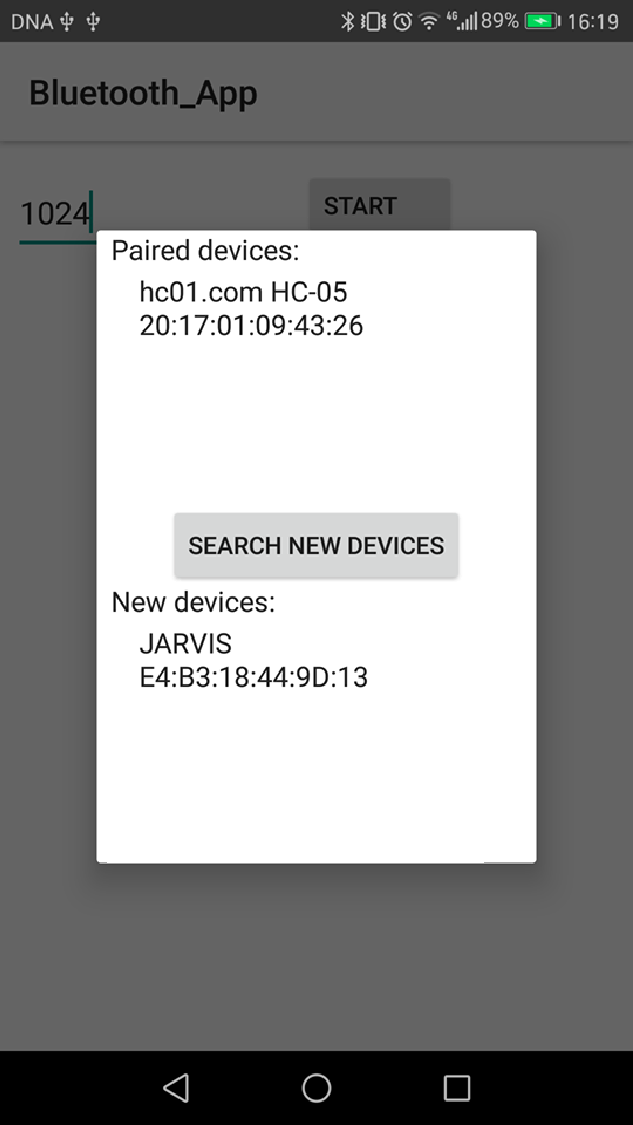
\includegraphics[scale=0.4]{images/app3layout.pdf}
		\caption{Bluetooth menu}\label{fig:btmenu}
	\end{minipage}
\end{figure}

	\subsection{Bluetooth application}
In the next two apps, we will transfer the matrics over to the SoC that will perform the matrix multiplicaiton. First, we'll explain how the Bluetooth app works.\\
Since this app works with bluetooth, we have to set up the permissions for the app to use the phone's Bluetooth adapter in the AndroidManifest.xml file like so:\\\\
\indent	$<$uses-permission android:name="android.permission.BLUETOOTH\_ADMIN"/$>$
\indent $<$uses-permission android:name="android.permission.BLUETOOTH"/$>$
\\\\
The first thing the app will do is check wether or not your phone's Bluetooth is enabled. If not, it will ask you if you want to enable the Bluetooth. If you press allow, you'll be directed to the main screen. If the Bluetooth was already enabled, nothing will pop up and you'll see the main screen in front of you. The front end of the app is simple, consisting of only one textview and two buttons. The textview has the purpose to allow you to input a custom size for your matrix's row and column. The first button "Start" will make 2 matrices with the given size. The other button will open a menu with 2 lists and a third button. The first list will show you all the already paired Bluetooth devices on your phone. The other list is empty, but after pressing the button "Search new devices", the list will fill up with discoverable devices around you as you can see in figure \ref{fig:btmenu}.Tapping on one of the new devices will result in an attempt to pair with this device. Tapping on a paired device in the list will result in an attempt to connect to that device. The device you selected will be the device you will communicate with. Android Studio provides libraries that easily gives you acces to the Bluetooth adapter in the phone. More information on how the Bluetooth adapter works can be found on the Android developer website \cite{AndroidDeveloper}. When the connection is established, the protocol described in \ref{subsec:bluetoothProtocol} will be executed.\\
The Bluetooth adapter has an in- and an outputstream to respectively read and write data. 
Both of which run in a thread so whenever there is new data coming from the SoC, the app will be able to read that. The received messages go to the message handler. In this message handler, various things happen depending on which message was received. Some of the effects of the messages are described in \ref{subsec:bluetoothProtocol} and here we'll explain what happens in the background of the app.\\
Listing \ref{lst:bluetoothHandler} is a piece of the handler code. First, we set up some byte array variables. One of these will read and copy whatever is in the buffer, while the other is used to make our messages send to the SoC. The following if-statement asks if the phone is the device that is currently "sending" matrices. If so, a second if-statement awaits with cases for all possible messages the phone can receive from the SoC. As we already know, when the phone receives the message "C", we will be starting to send over the matrices. We define an integer "i" that functions as an index to go through the matrix that contains the messages we have to send. We define a new message with the first element of the array and we define a first timestamp that indicates the beginning of the whole process. Next up is the "O" message. This message is received whenever the SoC acknowledges that it has received our previous data. We increment our index and check if the index is not exceeding our matrix length. If the index is ok, we send a message with the next array component. When the SoC didn't receive our message correctly, we should receive the message "R". If this is the case we will not increment the index so it will just send the previous message again. As for now, we only send one matrix over to the SoC for the sole purpose of testing the transmission time since sending the second matrix would take the same amount of time because they have the same size. Whenever the matrix has been transfer, the SoC will send an "X". At that point we make another timestamp so we know the elapsed time for sending one matrix from the phone to the SoC. The time will be printed in the log with the code shown in listing \ref{lst:bluetoothPrint}. In the meanwhile, the phone sends a message "C" to the SoC in order to switch the roles. The SoC will become the transmitter and the phone will act as a receiver.

\begin{lstlisting}[caption={Bluetooth message handler as transmitter},captionpos=b, label={lst:bluetoothHandler}, language=java, float=ht]
 1| byte[] readBuf = (byte[]) msg.obj;
 2| byte[] newMsg;
 3| String readMessage = new String(readBuf, 0, msg.arg1)
 4| if(sending){
 5|   if (readMessage.equals("C")) {
 6|     i = 0;
 7|     newMsg = (String.valueOf(matrixD[i]) + ":").getBytes();
 8|     t1 = System.currentTimeMillis();
 9|   }else if (readMessage.equals("O")) {
10|     i++;
11|     if(i<matrixD.length){
12|       newMsg = (String.valueOf(matrixD[i]) + ":").getBytes();
13|     }
14|   }else if (readMessage.equals("R")) {
15|     newMsg = (String.valueOf(matrixD[i]) + ":").getBytes();
16|   }else if (readMessage.equals("X")) {
17|     t2 = System.currentTimeMillis();
18|     newMsg = "C".getBytes();
19|     printTime();
20|     i = 0;
21|   }
22|   else{
23|     newMsg = ":".getBytes();
24|   }
25| mChatService.write(newMsg);
\end{lstlisting}


\begin{lstlisting}[caption={Prints elapsed time for sending matrices},captionpos=b, label={lst:bluetoothPrint}, language=java, float=hbtp]
1| public void printTime(){
2|   Log.i(TAG, "---------------------------------------------");
3|   Log.i(TAG, "Time = " + String.valueOf(t2 - t1));
4|   Log.i(TAG, "---------------------------------------------");
5| }
\end{lstlisting}

Listing \ref{lst:bluetoothHandler2} starts of with the else-statement that is related to the if-statement from listing \ref{lst:bluetoothHandler}. Now that the phone is the receiver the first message we would receive from the SoC should be a "D", indicating the SoC is done with the matrix multiplication. We send over message "C" to tell the SoC that the phone is ready to receive data. We also set up a timestamp to indicate the beginning of the receive time. Further messages that will be received will be a set of numbers with a ":"-symbol at the end to indicate that it is the end of the message. In subsection \ref{subsec:bluetoothProtocol} we explain why we do this. If the received number follows the rules of the protocol we confirm that we received the number correctly by sending an "O" as a message to the SoC. In case we suffered from data loss or any other error, we send an "R". Line 10 in listing \ref{lst:bluetoothHandler2} will check wether or not our matrix is full. If that is the case we make a second timestamp and print the time it took to receive te matrix.

\begin{lstlisting}[caption={Bluetooth message handler as receiver},captionpos=b, label={lst:bluetoothHandler2}, language=java, float=ht]
 1| else{
 2|   if(readMessage.equals("D")){
 3|     newMsg = "C".getBytes();
 4|     t1 = System.currentTimeMillis();
 5|   }else if(readMessage.length()==wordSize+1 && readMessage.endsWith(":")){
 6|      try{
 7|       matrixC[counter] = Integer.parseInt(readMessage.substring(0, wordSize));
 8|       counter++;
 9|      }catch(Exception e){}
10|       if(matrixC[elements-1] != null){
11|         t2 = System.currentTimeMillis();
12|         printTime();
13|       }
14|       newMsg = "O".getBytes();
15|   }
16|   else{
17|     newMsg = "R".getBytes();
18|   }
19|   mChatService.write(newMsg);
20| }
\end{lstlisting}

	\subsection{WebSocket application}\label{subsec:webapp}
Just like in the Bluetooth application, the SoC has to solve the matrix multiplication. Again, the front end of the app is really simple, containing only a textview and a button (figure \ref{fig:app1layout}). The textview is for defining a matrix size for the rows and columns. With the first tap on the button, you confirm the matrix size and create 2 square matrices with the chosen size containing random values from 0 to 99. The second tap will connect you to the WebSocket whos IP address is predefined as you can see in line 4 of listing \ref{lst:webSocketClient}. In order for us to connect the phone to the WebSocket server, we need to create a WebSocket client first. The WebSocket client can be created with the code shown in listing \ref{lst:webSocketClient}. For the WebSocket client, we used the "org.java-websocket:Java-WebSocket:1.3.0" library since it is good and easy to use. Also, to allow the app to use the phone's internet connection, we have to put the following line in the AndroidManifest.xml file:\\\\
\indent $<$uses-permission android:name="android.permission.INTERNET"/$>$
\\\\
Now, whenever we call the method to initiate the WebSocket client, the URI from the server is required (line 4).  Line 9-50 are shown in listing \ref{lst:detailWebSocketClient} that gives the detailed code on which methods the socket has to contain in order to function properly. In line 51 we try to establish a connection between the client and the server.
\begin{lstlisting}[caption={Making a WebSocket client},captionpos=b, label={lst:webSocketClient}, language=java, float=h]
 1| public void connectWebSocket() {
 2|   URI uri;
 3| try {
 4|   uri = new URI("ws://130.230.144.40:8080");
 5| } catch (URISyntaxException e) {
 6|   e.printStackTrace();
 7|   return;
 8| }
 9|   socket = new WebSocketClient(uri, new Draft_17()) {...};
51|   socket.connect();
52| }
\end{lstlisting}\\
The socket requires certain methods that are invoked on a call from the server. For example, if the client connects succesfully with the server, method "OnOpen" is invoked. In this method we print a message to our Log that the phone succesfully connected to the server. The second method required for the WebSocket client is "onMessage". This method is invoked whenever the client receives a message from the server. What happens next depends on the message this method received. All different types of messages are put into an if-statement so we execute different code depending on the received message. You can read more about the messages on line 16, 19 and 23 in subsection \ref{subsec:websocketProtocol} where the transmission protocol is explained. If we receive "matrixA=" or "MatrixB=", we respectively start transferring matrix A and matrix B. But before we start sending them over, we create a timestamp t1 that will measure the system time in milliseconds at that point. We do the same thing for t2 as soon as we start sending matrixB. Having a timestamp for matrixB seems redunant but why this is done will be explained in the results. A third timestamp t3 is defined after receiving the message "matrixR=" which will represents the start of receiving data. The message in the next case is to determing how long the SoC's execution time was over calculating the matrix multiplication. When we receive message "done :D", we measure out last timestamp and close our WebSocket connection.

\begin{lstlisting}[caption={Detailed look at creating the WebSocket client},captionpos=b, label={lst:detailWebSocketClient}, language=java, float=h]
 9| socket = new WebSocketClient(uri, new Draft_17()) {
10|   @Override
11|   public void onOpen(ServerHandshake serverHandshake) {
12|     Log.i(TAG, "Connected to: " + uri.getHost() + ":" + uri.getPort());
13|   }
14|   @Override
15|   public void onMessage(String s) {
16|     if(s.equals("matrixA=")){
17|       t1 = System.currentTimeMillis();
18|       sendMatrixA();
19|     }
20|     else if(s.equals("matrixB=")){
21|       t2 = System.currentTimeMillis();
22|       sendMatrixB();
23|     }
24|     else if(s.equals("matrixR=")){
25|       t3 = System.currentTimeMillis();
26|     }
27|     else if(s.contains("Execution time in")){
28|       exeTime=s;
29|     }
30|     else if(s.equals("done :D")){
31|       t4 = System.currentTimeMillis();
32|       displayTimes();
33|     }
34|     else{
35|       try{
36|         int i = Integer.parseInt(s);
37|         matrixC[counter] = i;
38|         counter++;
39|       } catch(Exception e){}
40|     }
41|   }
42|   @Override
43|   public void onClose(int i, String s, boolean b) {
44|     counter = 0;
45|   }
46|   @Override
47|   public void onError(Exception e) {
48|     //Log.i(TAG, "Error " + e.getMessage());
49|   }
50| };
\end{lstlisting}

\chapter{Results}

\section{Phone performance}
In this section we will describe the performance and the results we got from our applications from section \ref{sec:AndroidApps}. The phone we used is a Huawei P9 (EVA-L09) that has following specifications:
\begin{itemize}
	\item{CPU: HiSilicon Kirin 955 2.52 GHz}
	\item{RAM: 2780MB}
	\item{Android version: 7.0}
\end{itemize}

	\subsection{Matrix multiplication}
The Huawei P9 is quite a powerful device and was able to outperform the SoC when calculating with medium sized matrices. When the app is executed correctly the screen should look like figure \ref{fig:app1Result}. While testing, we came accros some interesting findings when calculating matrices with the size of 1024. The time it took skyrockets when the matrix has an exact size of 1024. One column/row more or less and the app would behave as expected. From there on, the time for certain matrix sizes is inconsistent. Because we work with large matrices, we can hardly determine wether or not the phone is executing everything correctly making the results in figure \ref{fig:app1Graph} for large matrices unreliable.\\
Figure \ref{fig:app1usage} shows us the CPU and RAM usage over time. In the RAM graph we can clearly see where the matrices are generated. Over time the RAM usage increases and it drops after all matrices in the app are cleared. The CPU usage is around 12-13\% throughout the whole process.


\begin{figure}[ht]
	\begin{minipage}[t]{0.4\textwidth}
	\centering
	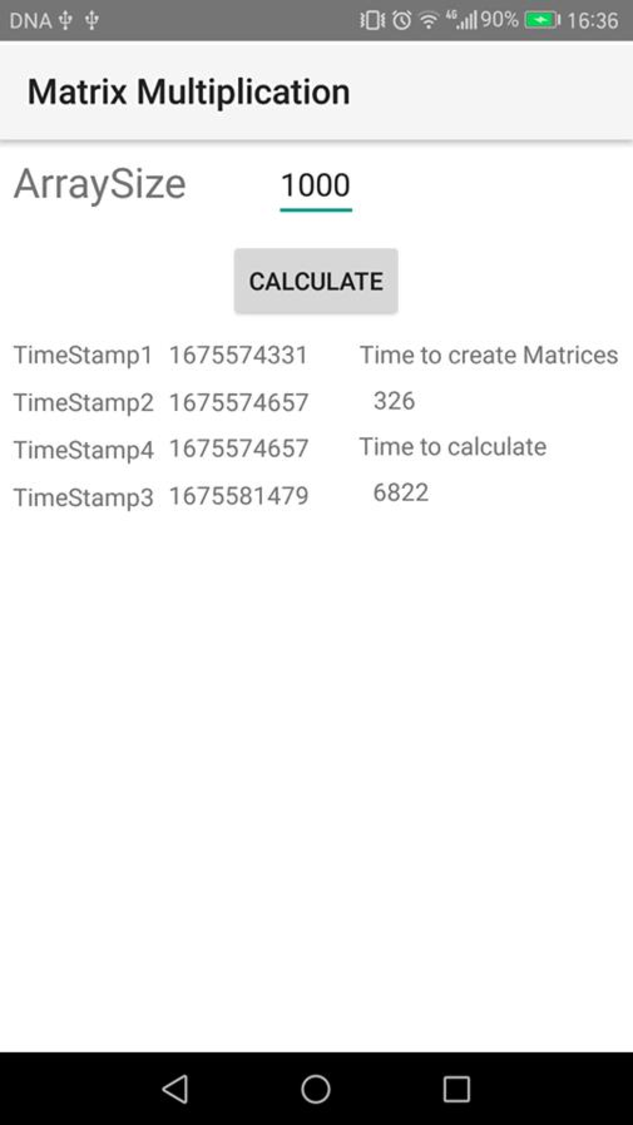
\includegraphics[scale=0.3]{images/app1result.pdf}
	\caption{Result screen matrix multiplication}\label{fig:app1Result}
	\end{minipage}
	\begin{minipage}[t]{0.5\textwidth}
	\centering
	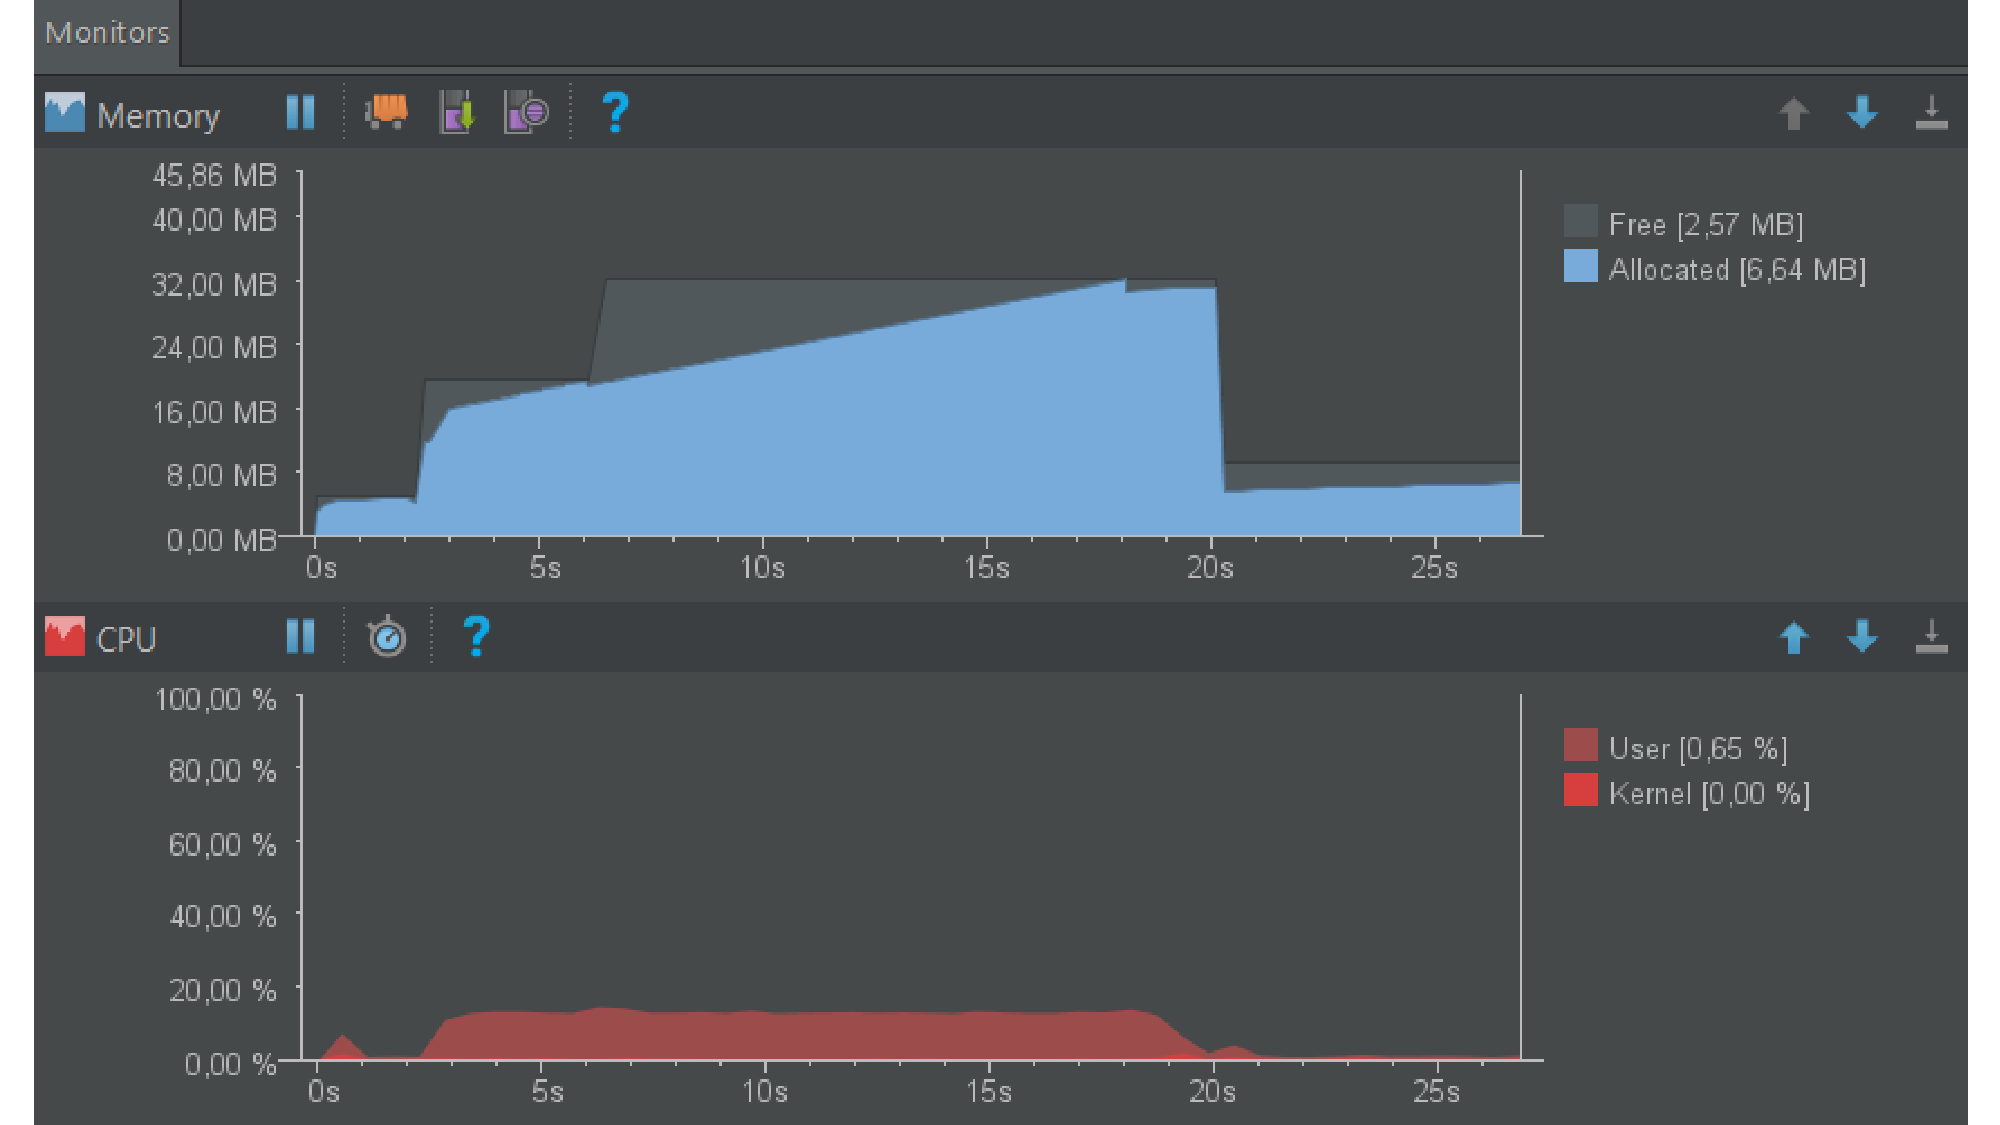
\includegraphics[scale=0.3]{images/app1usage.pdf}
	\caption{CPU and RAM usage}\label{fig:app1usage}
	\end{minipage}
\end{figure}


\begin{figure}[ht]
\centering
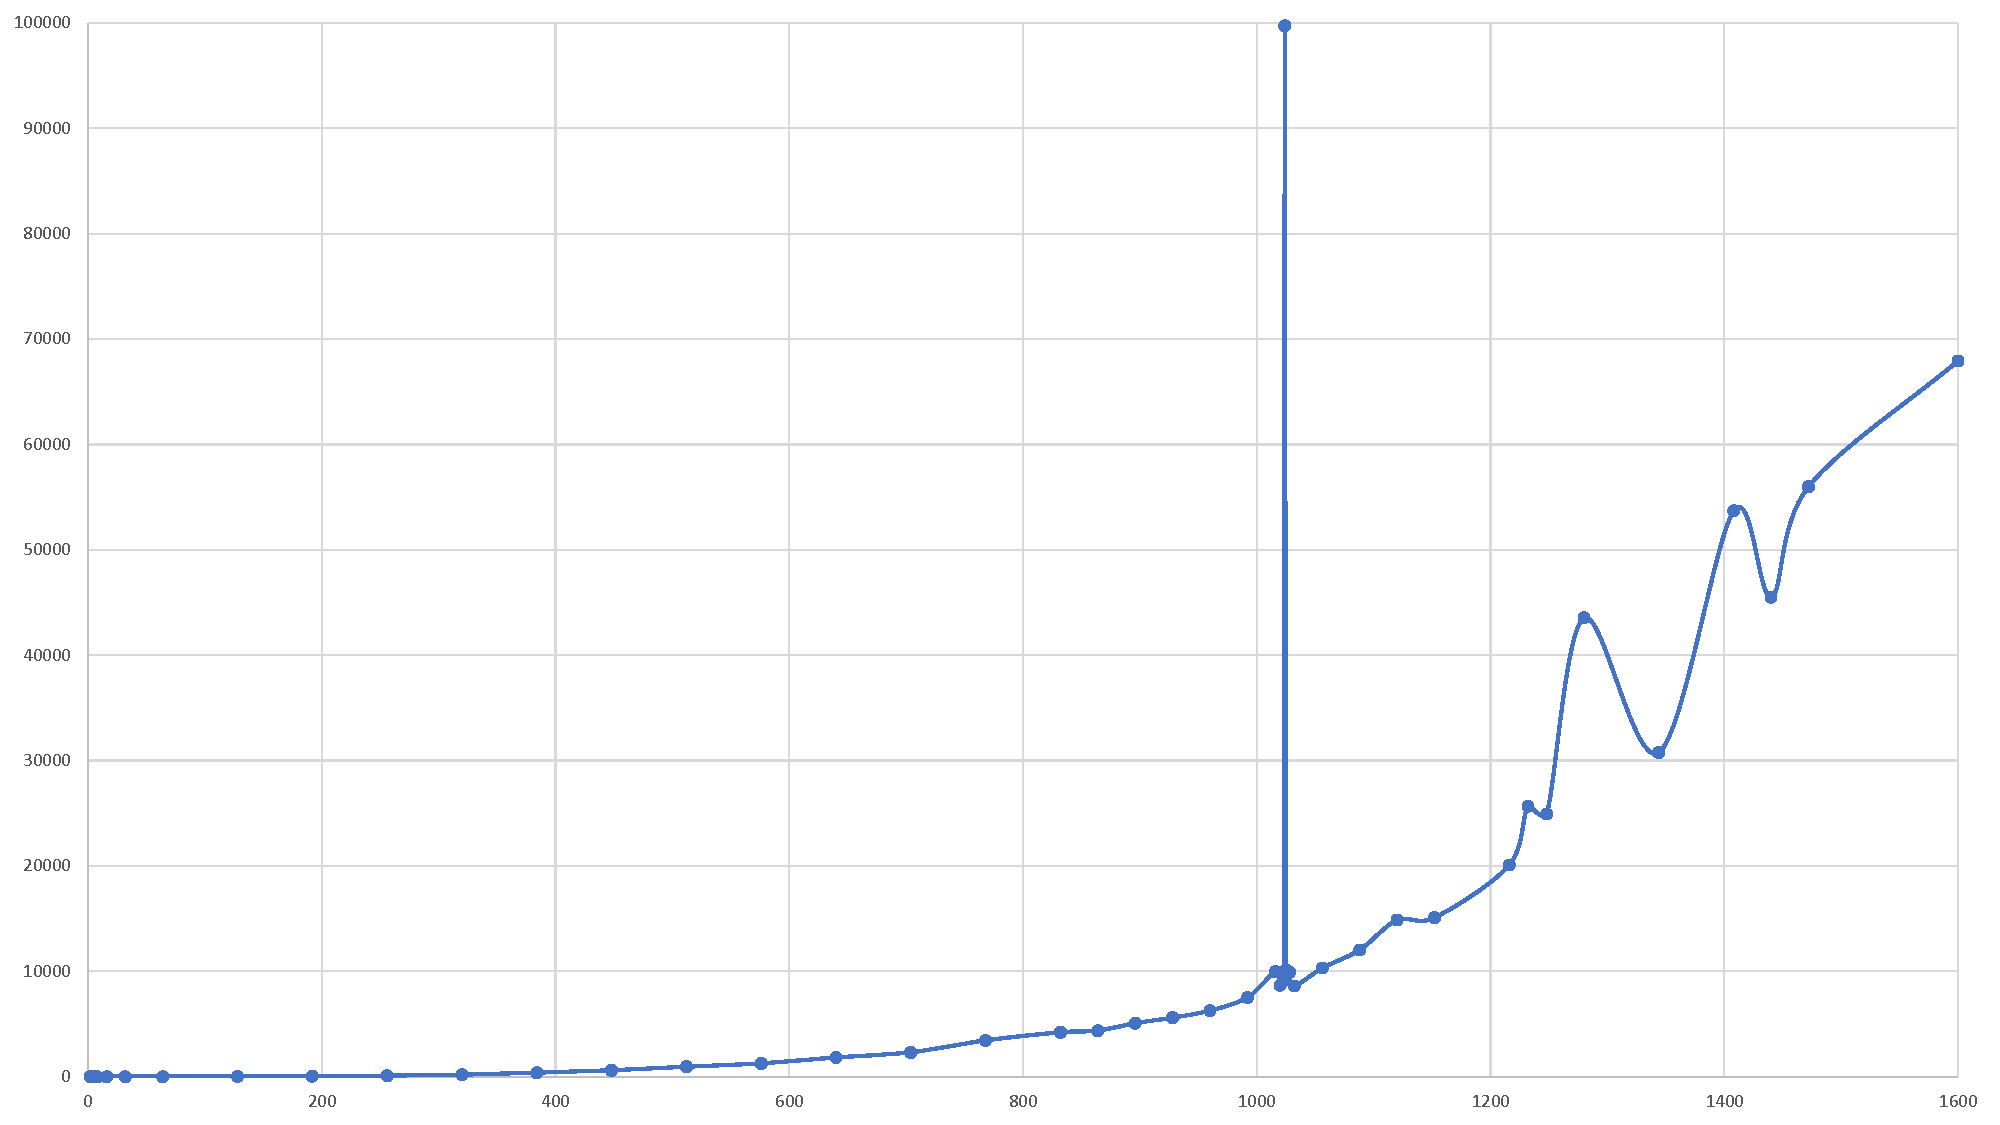
\includegraphics[scale=0.35]{images/app1graph.pdf}
\caption{Results matrix multiplication}\label{fig:app1Graph}
\end{figure}



	\subsection{Bluetooth app}
After connecting the devices, the SoC will request for the transmission of the data. There is not a lot happening in the front end but the transmission time and receive time are displayed in the Logcat like in figure \ref{fig:app3log} when the full process is done. Again we will check out the CPU and RAM usage of the app as we did with the previous app. If we look at figure \ref{fig:app3usage} we notice a lot of changes. The app barely uses and CPU power and also only requires a small amount of RAM to create the matrices. As for the Bluetooth app we were only able to test matrices that were smaller than 20x20 as the SoC would give the error: "Too many files open".

\begin{figure}[ht]
\centering
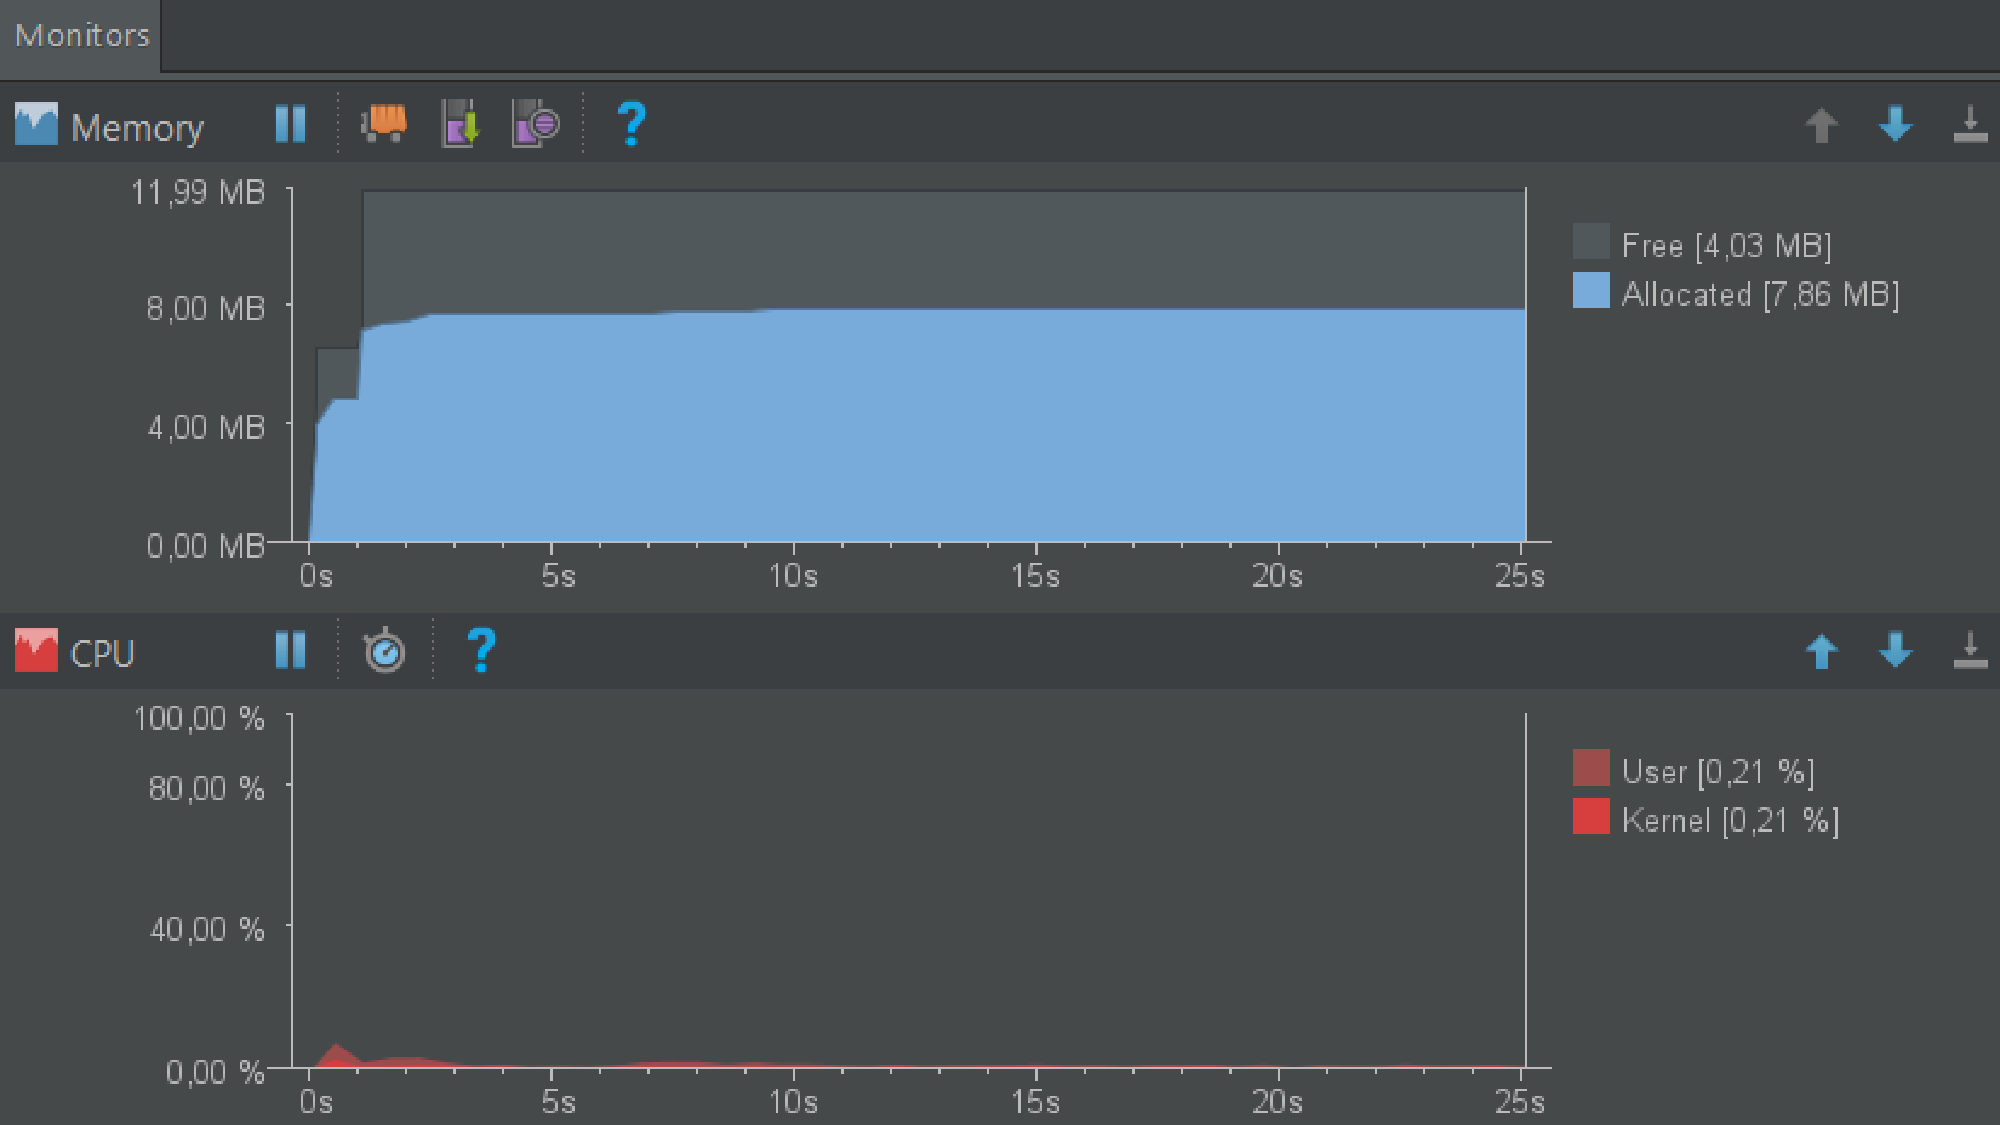
\includegraphics[scale=0.3]{images/app3usage.pdf}
\caption{CPU and RAM usage Blueooth}\label{fig:app3usage}
\end{figure}

\begin{figure}[ht]
\centering
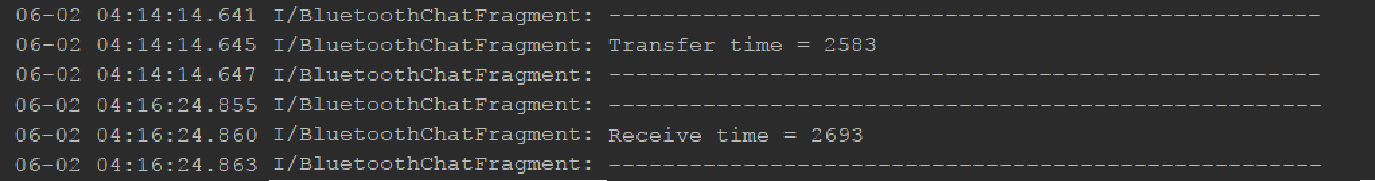
\includegraphics[scale=0.5]{images/app3Log.pdf}
\caption{Bluetooth app log}\label{fig:app3log}
\end{figure}

	\subsection{WebSocket app}
As for the WebSocket, there is a little more interesting data to show. If we look at the RAM usage in figure \ref{fig:app2usage}, the first increase in RAM is the app startup. The next one is where we create the matrices. Around 8 seconds the matrices are created and the network graph indicates we are transmitting the matrices over to the SoC. The decrease around 18 seconds indicates that we clear the matrices that have been send. After that we are in an idle state where we sent the last few messages that are in the WebSocket queue. When the SoC executed the multiplication it will send the solution back to the phone, hence the receive (Rx) spikes in the network graph. When we look at the CPU, it is mostly used when we receive data from the SoC. This is probably CPU intensive since we slowly fill up the solution matrix with the data that is received from the SoC.\\
The log file in figure \ref{fig:app2log} shows all time intervals mentioned in \ref{subsec:webapp}.

\begin{figure}[hbtp]
\centering
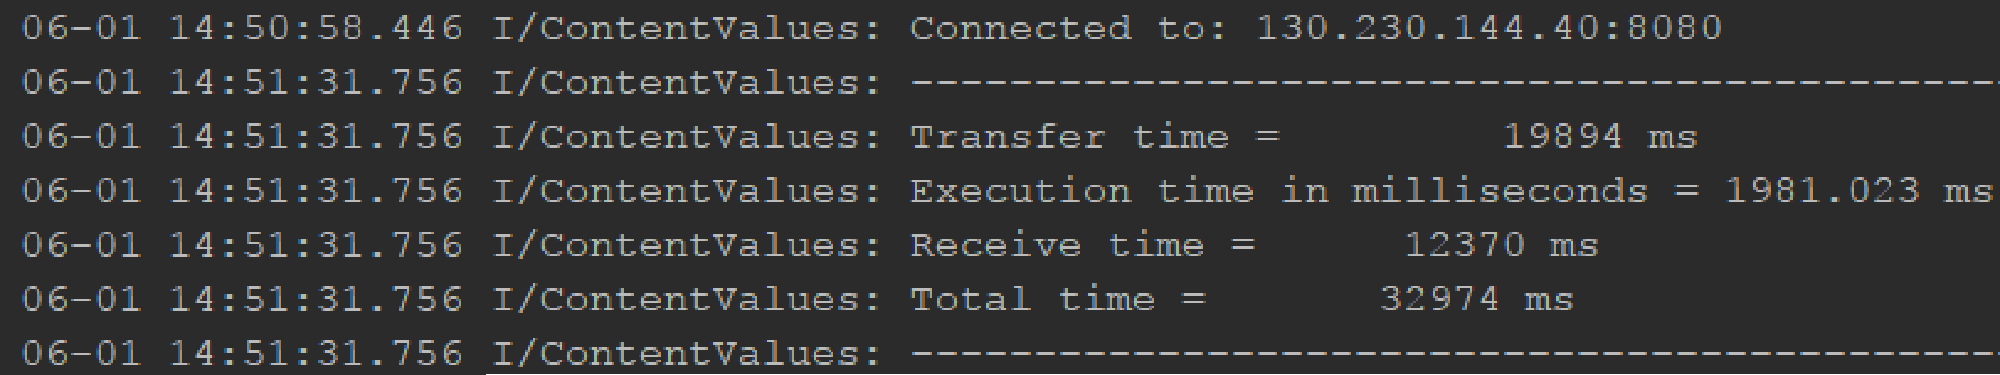
\includegraphics[scale=0.35]{images/app2resultlog.pdf}
\caption{WebSocket app log}\label{fig:app2log}
\end{figure}

\begin{figure}[hbtp]
\centering
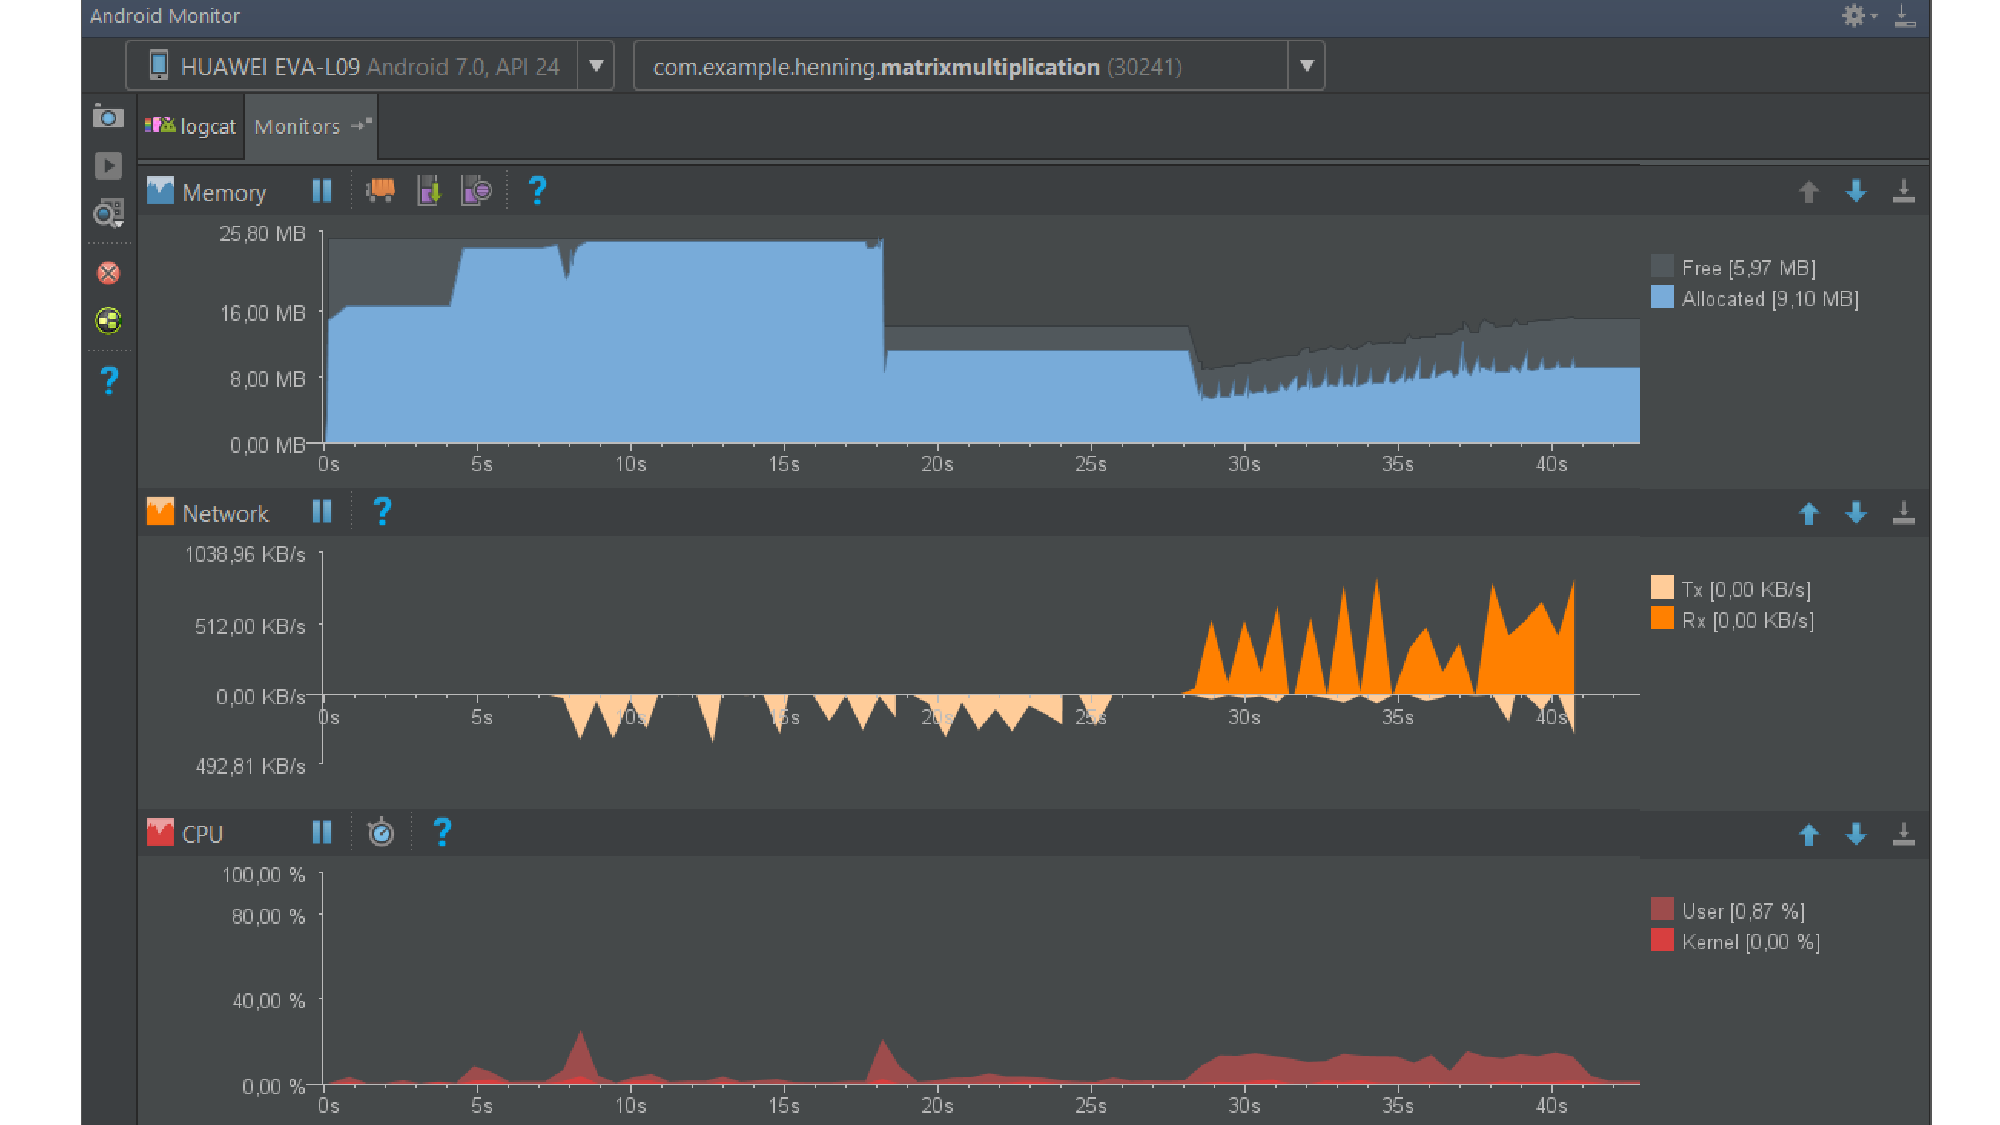
\includegraphics[scale=0.35]{images/app2resultgraph.pdf}
\caption{CPU, RAM and network usage WebSocket}\label{fig:app2usage}
\end{figure}

\section{Bluetooth vs web socket communication speed}
In order to choose the best communication protocol, we have to test both Bluetooth and WebSocket communication preferable with large sized arrays. First, we perform the actual communication in order to find a relation between the arraysize and the elapsed time. When we find this relation we can set up a formula that allows us to calculate an estimate value for the elapsed time for any matrix size.

	\subsection{WebSocket transmission}
We first performed multiple calculations with WebSocket communication. We seperated the elapsed time it took the phone to transmit the data and the elapsed time it took the SoC to transmit the data. If we divide the total number of seperate symbols in one matrix with the elapsed time, we know the amount of symbols that are transmitted per second (sym/s). For small matrices, the sym/s is not reliable since there are background processes that influence these results. Although, these background processes barely affect the sym/s with larger matrices. So in order to determine the relation, we will take an average of all the sym/s with all matrix sizes, apart from those that are highly affected by background processes. This resulted in a sym/s value of 86843,61 for the phone transmission and 127228,7 for the SoC transmission. Knowing these values we can make graph \ref{graph:websocketTime}. In the graph we compare the transmission time for the phone with the time for the SoC. The small dent in 
the SoC curve is the change in average number length in the matrix from 6 to 7.
\begin{figure}[ht]
\centering
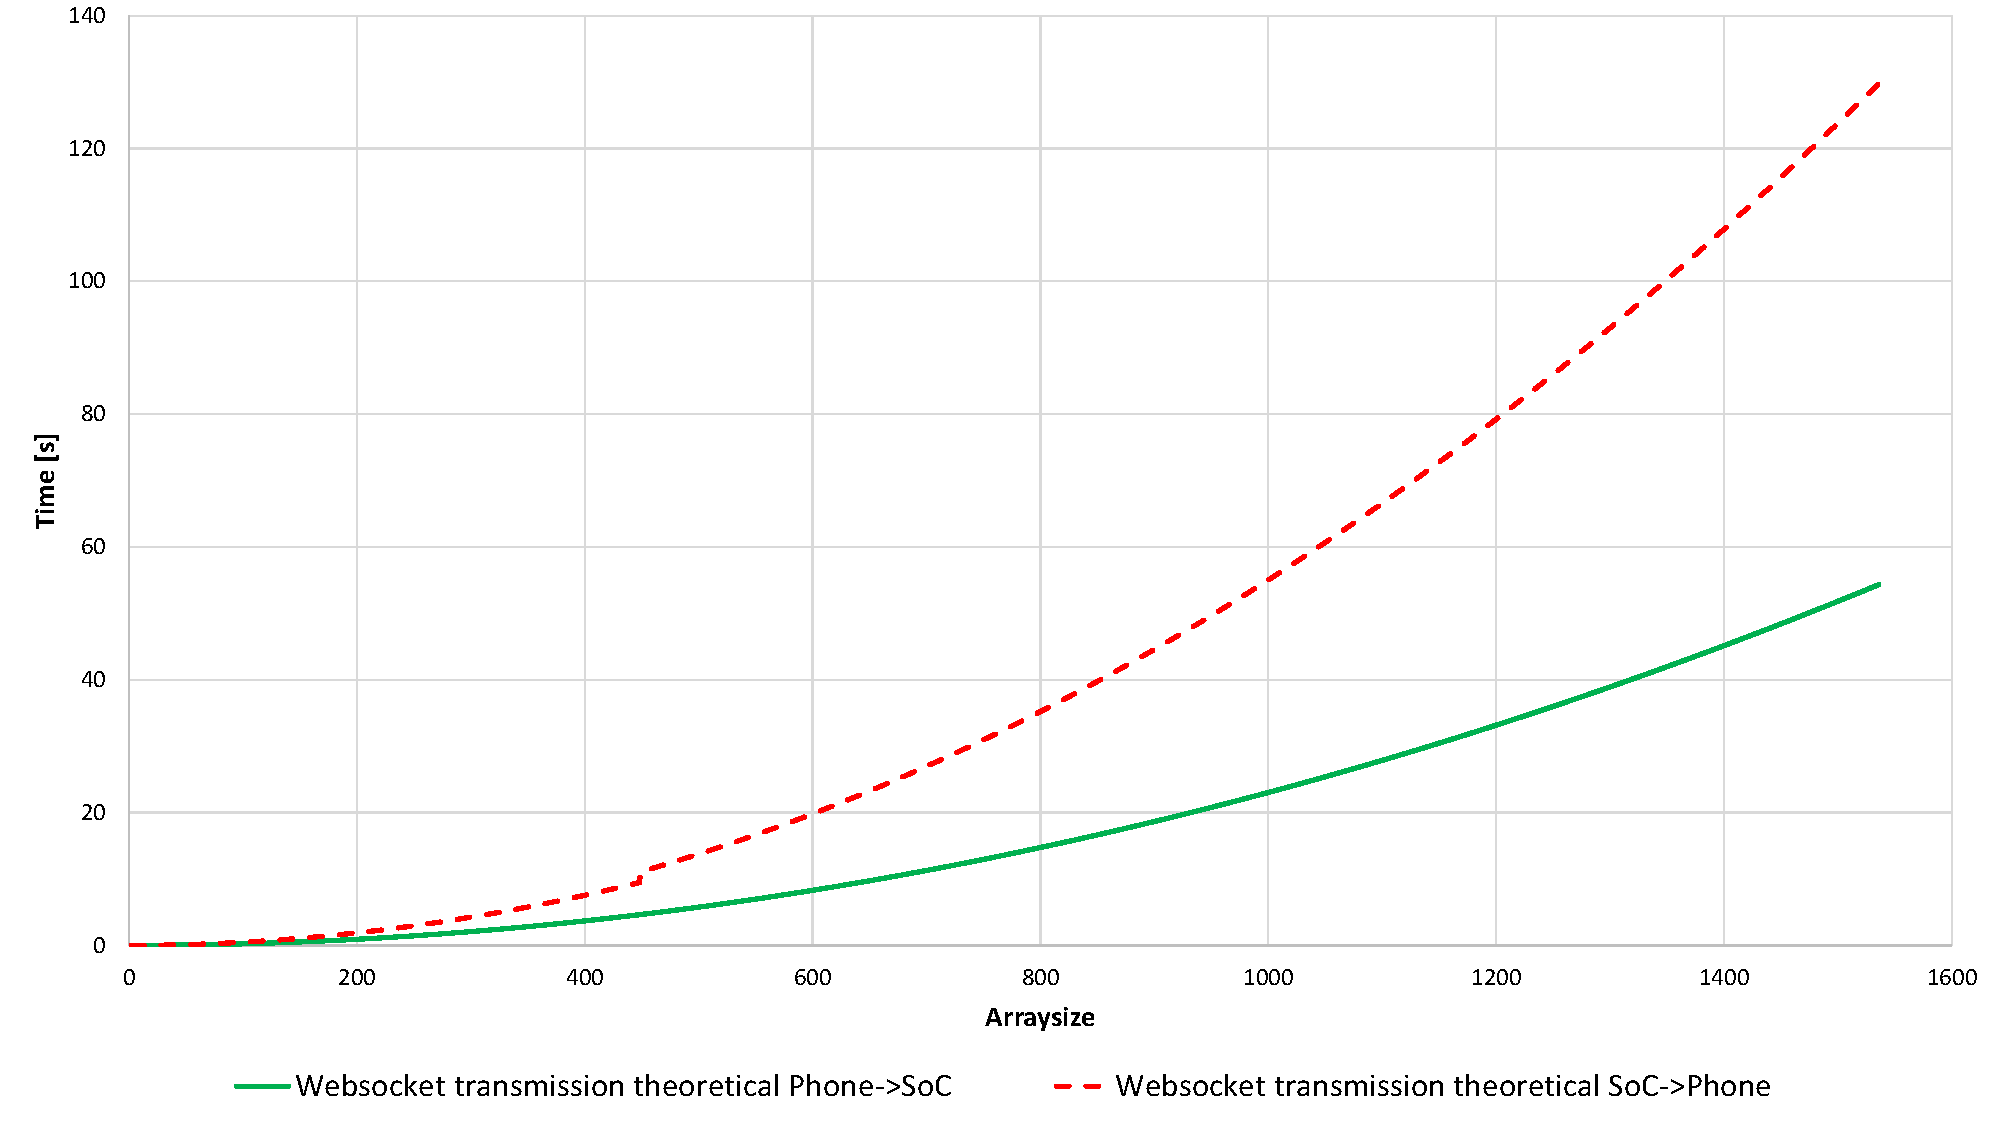
\includegraphics[scale=0.45]{images/WebsocketTransmissionSpeed.pdf}
\caption{WebSocket transmission time for phone to SoC and vice versa}\label{graph:websocketTime}
\end{figure}

\subsection{Bluetooth transmission}
Next we determine the transmission time using the Bluetooth communication. We only mention the practical elapsed time to send over one matrix from the phone to the SoC the elapsed time the other way around was very similar. We were only able to test small matrices of up to a size of 20x20. The sym/s for this communication protocol was around 258 sym/s including a lot of repeated messages due to package loss. Although we are not able to transfer large matrices, we are able to set up a formula that allows us to make an estimate of the elapsed time for higher matrices. The results for this are shown in graph \ref{graph:bluetoothTime}.

\begin{figure}[ht]
\centering
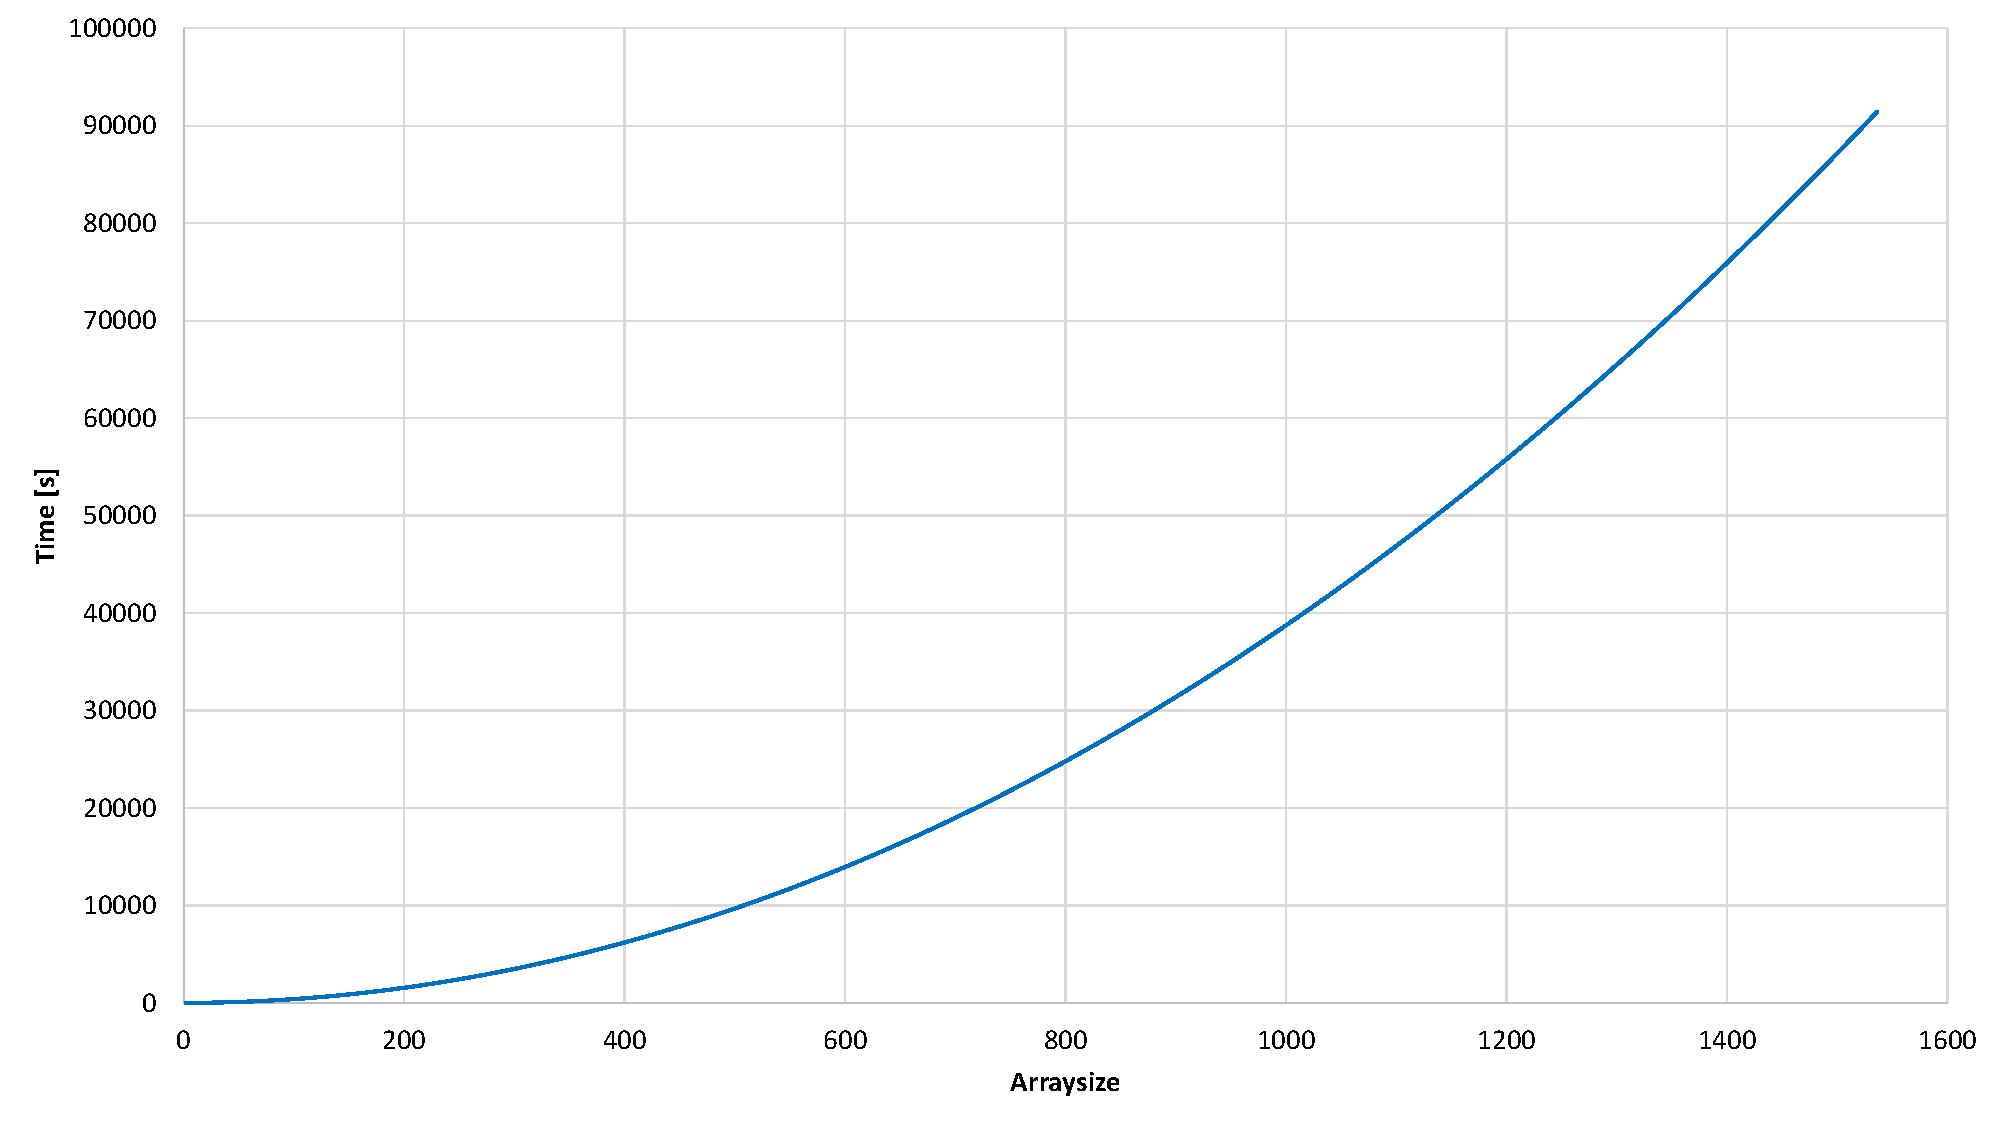
\includegraphics[scale=0.45]{images/BluetoothtransmissionSpeed.pdf}
\caption{Bluetooth transmission time}\label{graph:bluetoothTime}
\end{figure}

\subsection{Bluetooth vs. WebSocket}
Comparing the sym/s and looking at both graph scales, it is very clear that the WebSocket is way more faster than Bluetooth communication. The WebSocket transfer time from the phone to the SoC is around 340 times faster while vice versa the WebSocket is almost 500 times faster. The WebSocket also allowed us to practically transfer much larger matrices aswell making it superior compared to our Bluetooth communication. Graph \ref{graph:bluetoothVsWebsocket} visualizes the difference in scale for both communication protocols. We can clearly see that the WebSocket requires less time to transfer one matrix compared to Bluetooth.

\begin{figure}[ht]
\centering
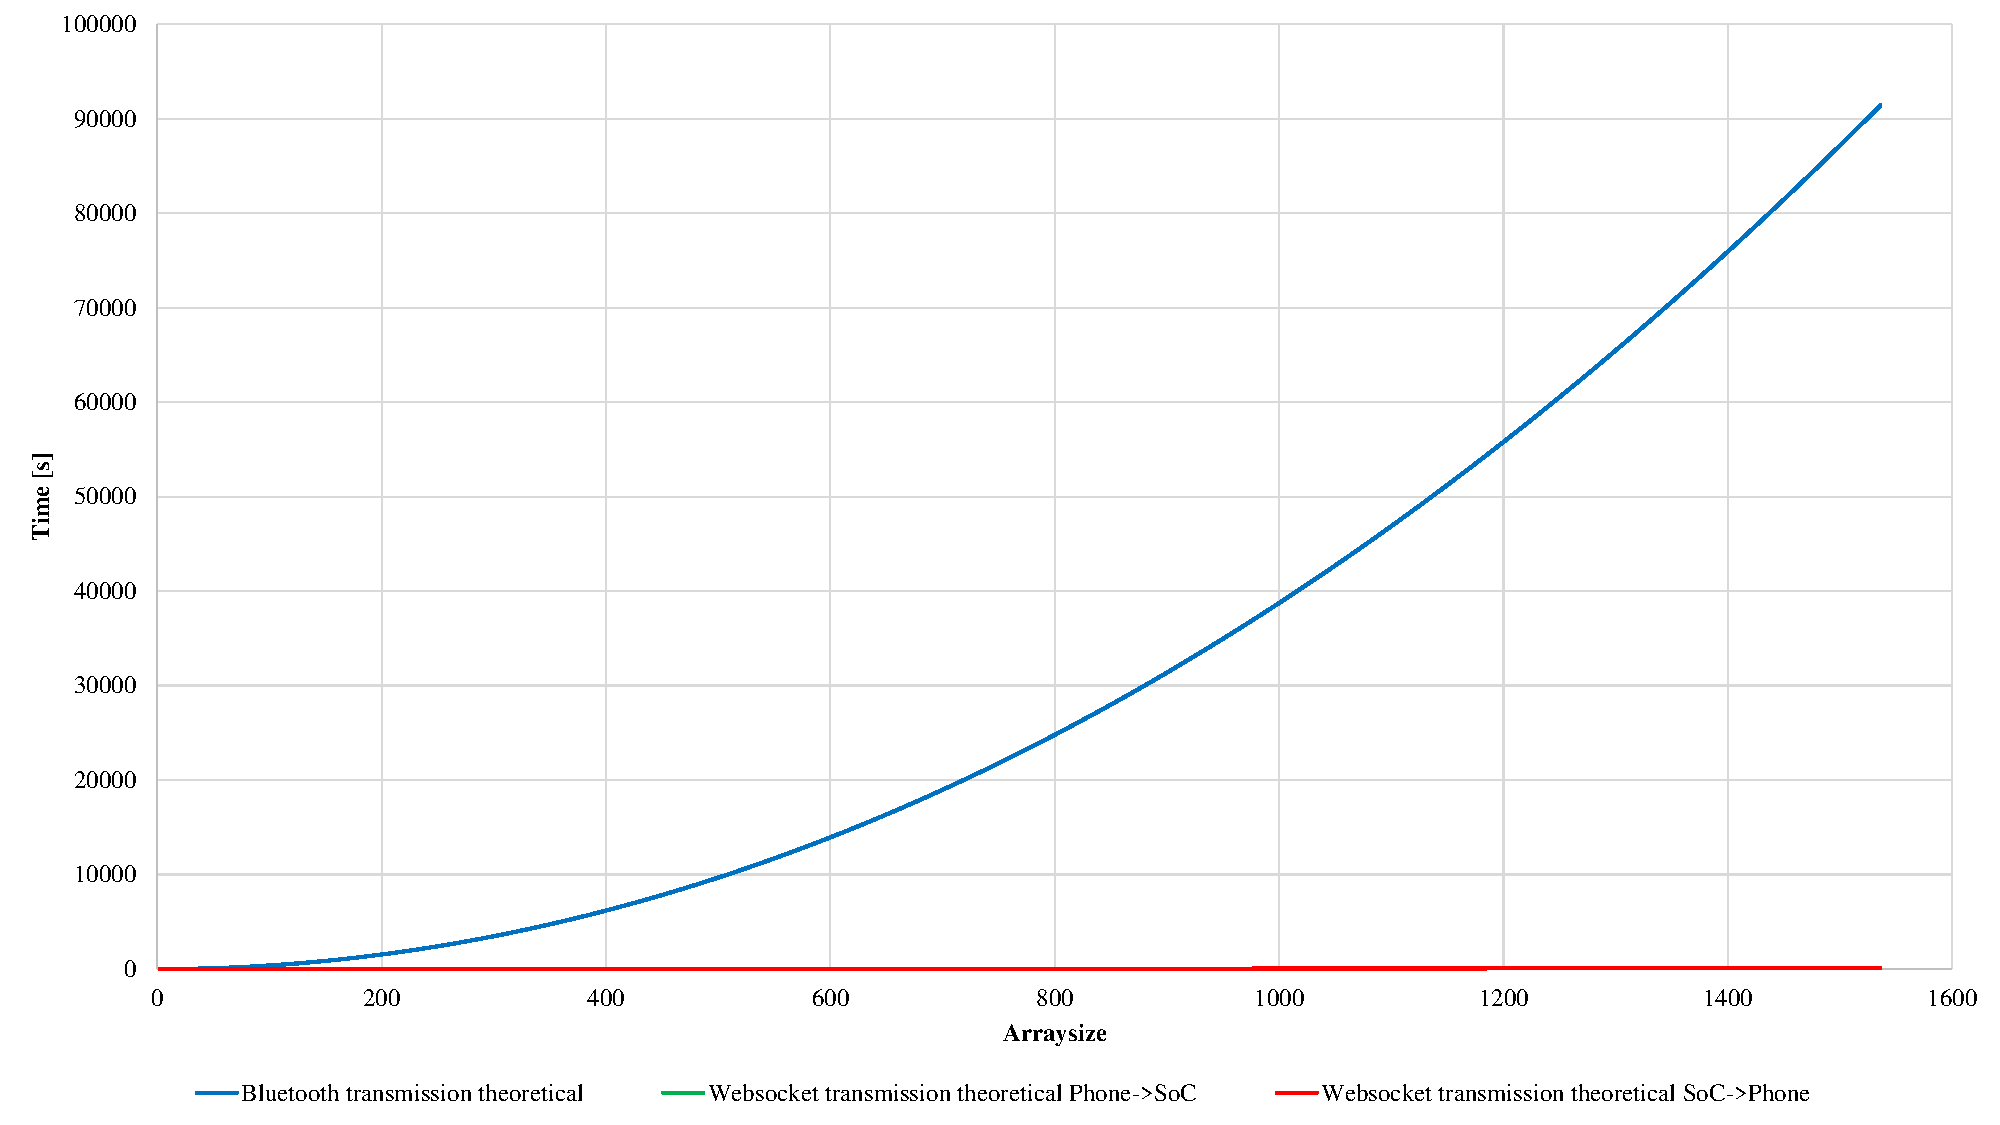
\includegraphics[scale=0.45]{images/BluetoothVsWebsocket.pdf}
\caption{Bluetooth transfer time vs. WebSocket transfer time}\label{graph:bluetoothVsWebsocket}
\end{figure}

\subsection{WebSocket and SoC vs. Android smartphone}
As discussed in previous subsection, we can conclude that there is no way of Bluetooth being worthwhile for this project. Thus, we are only testing the WebSocket protocol combined with the SoC's ability to multiply matrices. Subsection \ref{subsec:compArch} gives us a comparison between the phone and the SoC on how fast they can process the matrix multiplication. Now we want to know at which point the Android phone will be slower than transferring all three matrices and performing the matrix multiplication on the SoC. If we look back at graph figure \ref{grap:openclCalcu}, the orange curve represents the estimate of the total transfer time of all three matrices. While the yellow and gray curves respectively represent the calculation time it takes to perform the multiplication with the SoC and the Mac. The yellow and gray curves are trendlines derived from data we achieved from performing multiple matrix multiplications with different matrix sizes. The equation for the yellow curve trendline is equation \ref{eq:trendlineGlobalSoC} and the grey curve's trendline is equation \ref{eq:trendlineGlobalMac}. Combining these gives us the blue curve which represents the combination of the transfer time and the Mac calculation time, while the green curve shows the combination of the transfer time and the SoC calculation time. If we look at the green curve we see it crosses the black curve, which is the trendline made with equation \ref{eq:trendlineAndroid} around a matrix size value of 2350. If we want a more correct value for this we take a look at the equation that defines both curves. Equation \ref{eq:trendlineAndroid} represents the used function to generate the trend line of the Android phone execution time. Equation \ref{eq:totalTransferTime} is a combination of the data transfer time from both the phone and the SoC. The transfer speed from the phone is 43,42 numbers/second while the SoC can transfer the larger numbers back to the phone at a rate of 18,85 numbers/second. In order to find the the value for the matrix size where the phone execution time will be the same as the full process time from the SoC, we have to find x in y=v+w, with y equal to equation \ref{eq:trendlineAndroid}.

\begin{equation} \label{eq:totalCalcTimeSoC}
v = -3*10^{-10}*x^4+2*10^{-5}*x^3-0,0021*x^2-0,2801*x+142,83
\end{equation}

\begin{equation} \label{eq:totalTransferTime}
w = \frac{2*x^2}{43,42}+\frac{x^2}{18,85}
\end{equation}

if we extract x from y=v+w we get a value of 2338. This means we have an even time for both processes in case we try to do a matrix multiplication with two 2338x2338 matrices.


\bibliographystyle{IEEEtran}
\bibliography{References}
\end{document}
